\documentclass[11pt]{article}
\usepackage[margin=1in]{geometry}
\usepackage{amsmath,amssymb,amsthm,mathtools,booktabs,graphicx,microtype}
\usepackage[hidelinks]{hyperref}
\newtheorem{theorem}{Theorem}[section]
\newtheorem{lemma}[theorem]{Lemma}
\newtheorem{proposition}[theorem]{Proposition}
\newtheorem{corollary}[theorem]{Corollary}
\theoremstyle{definition}
\newtheorem{definition}[theorem]{Definition}
\theoremstyle{remark}
\newtheorem{remark}[theorem]{Remark}
\DeclareMathOperator{\osc}{osc}
\DeclareMathOperator{\sgn}{sgn}
\DeclareMathOperator{\artanh}{artanh}
\newcommand{\E}{\mathbb E}
\newcommand{\Prob}{\mathbb P}
\newcommand{\R}{\mathbb R}
\newcommand{\Vcl}{\mathcal V}
\newcommand{\reach}{\mathcal I}
\newcommand{\routing}{\mathcal R}
\newcommand{\full}{L_V}
\newcommand{\err}{|D_{2h}-L_V|}
\allowdisplaybreaks
\emergencystretch=2em
\title{Local Factor Graph Debate\\\large A mathematical companion}
\author{Codex, Claude}
\date{September 2026}
\begin{document}
\maketitle
\begin{abstract}
Two debaters know a graphical model that a judge can inspect only a little
at a time. They take turns choosing variables to reveal; the judge then
computes the target log-odds in the revealed submodel. How close is the
result to the answer from the whole model? We develop the argument in the
order of the accompanying post. A small set of arguments first gives a
strategic guarantee. Message passing then bounds the influence of everything
outside that set. Gaussian averaging turns this bound into a power of the
inspection budget. Finally, a projection argument on regular trees explains
why a polynomial obstruction can remain even under optimal play.
The guarantees concern agreement with the full model, and place no bound
on the computation used by the judge or the players.
\end{abstract}
\noindent\textit{Acknowledgments.} Stephan W\"aldchen, Dmitry Vaintrob, and
other collaborators contributed ideas to this project. Codex and Claude
were used to generate and develop proofs; this companion was prepared with
Codex. Mathematical arguments and numerical evaluations are distinguished
below. No claim of complete machine verification is made for this document.
\setcounter{tocdepth}{1}
\tableofcontents

\clearpage
\section{The question: how much must the judge see?}

Imagine a question surrounded by a large network of related claims.
Some claims bear directly on the question; others matter only because they
change how we interpret those nearby. Two informed advocates can each draw
the judge's attention to a few claims. If one argues for a high answer and
the other for a low answer, can either systematically exploit what remains
unseen?

The useful object will be a \emph{core}: a small collection of claims that
makes the answer stable under every further revelation. If either advocate
can insist on showing that collection, both acquire a way to constrain the
outcome. The equilibrium transcript need not contain it. A credible
alternative strategy already constrains a zero-sum game's value.

The rest of the argument asks when such a core exists. Along a chain of
weak interactions, the effect of a distant claim is repeatedly diminished.
Branching works in the opposite direction: there are more distant claims.
On a graph with maximum degree $d$, a radius of $R$ can cost on the order of
$(d-1)^R$ vertices. Thus exponential decay in distance becomes polynomial
decay in the number of revelations. This change of scale is the geometric
reason for the powers appearing later.

The connection with statistical mechanics is useful, but the model here
is more specific than an analogy with a magnet. A random interaction table
produces both an interaction and random local preferences. Strong local
preferences can suppress the transmission of additional evidence. Increasing
the scale of the tables therefore need not make debate harder.
Neither a failed upper bound nor a finite-budget numerical plateau proves a
phase transition. Nor is completion stability the same as weak spin
correlation: with zero fields and pure interactions $J_ex_ux_v/2$, global
spin-flip symmetry gives $L_S=0$ for every induced submodel. All core
oscillations then vanish, even when strong positive interactions make
spins highly correlated.

Debate as a method of supervision has a broader literature
\cite{irving,browncohen}. Here we isolate one mechanism: strategic selection
of authentic model components. We do not model fabricated evidence,
approximate optimization, or computationally limited inference.

\clearpage
\section{Problem formulation}
\label{sec:model}

\subsection{A revealed claim adds a variable}
Let $G=(V,E)$ be a finite simple undirected graph and $t\in V$ its target.
A variable $x_v\in\{-1,+1\}$ represents whether claim $v$ is false or true.
A vertex has a unary \emph{log-factor}
$\varphi_v:\{-1,+1\}\to\R$. An edge $\{u,v\}$ has a binary log-factor
$\theta_{(u,v)}:\{-1,+1\}^2\to\R$, with
\[
 \theta_{(v,u)}(b,a)=\theta_{(u,v)}(a,b).
\]
The reverse orientation names the same table. Each undirected edge is
counted once. Missing unary factors are represented by $\varphi_v=0$.
All factors are finite; very large unary contrasts can approximate hard
constraints, but infinite log-odds are outside our statements.

For a transcript $t\in S\subseteq V$, the judge uses
\begin{equation}
 P_S(x)=\frac1{Z_S}\exp\left\{
 \sum_{\substack{\{u,v\}\in E\\u,v\in S}}\theta_{(u,v)}(x_u,x_v)
 +\sum_{v\in S}\varphi_v(x_v)\right\},\qquad x\in\{-1,+1\}^S.
 \label{eq:model}
\end{equation}
Here $Z_S$ is the sum of the numerator over all assignments, so $P_S$ is a
probability distribution. Write
\begin{equation}
 L_S=\log\frac{P_S(x_t=+1)}{P_S(x_t=-1)}.
 \label{eq:logit}
\end{equation}
The reference answer is $L_V$, the log-odds from the entire model.

Revealing $v$ exposes its unary factor and all edge tables joining it to
already revealed vertices. It does not announce a value of $x_v$.
The judge's distribution is the \emph{induced submodel}: factors touching
unrevealed vertices are omitted. It is generally different from the marginal
of $P_V$ on $S$. For example, with energy $Jx_tx_u/2+\ell x_u/2$, deleting
$u$ gives target log-odds zero, whereas summing over $x_u$ gives
\[
 \log\cosh\frac{\ell+J}{2}-\log\cosh\frac{\ell-J}{2},
\]
which need not vanish. Selection itself is not treated as Bayesian evidence.
These are substantive assumptions about the judge.

\begin{figure}[htbp]
\centering
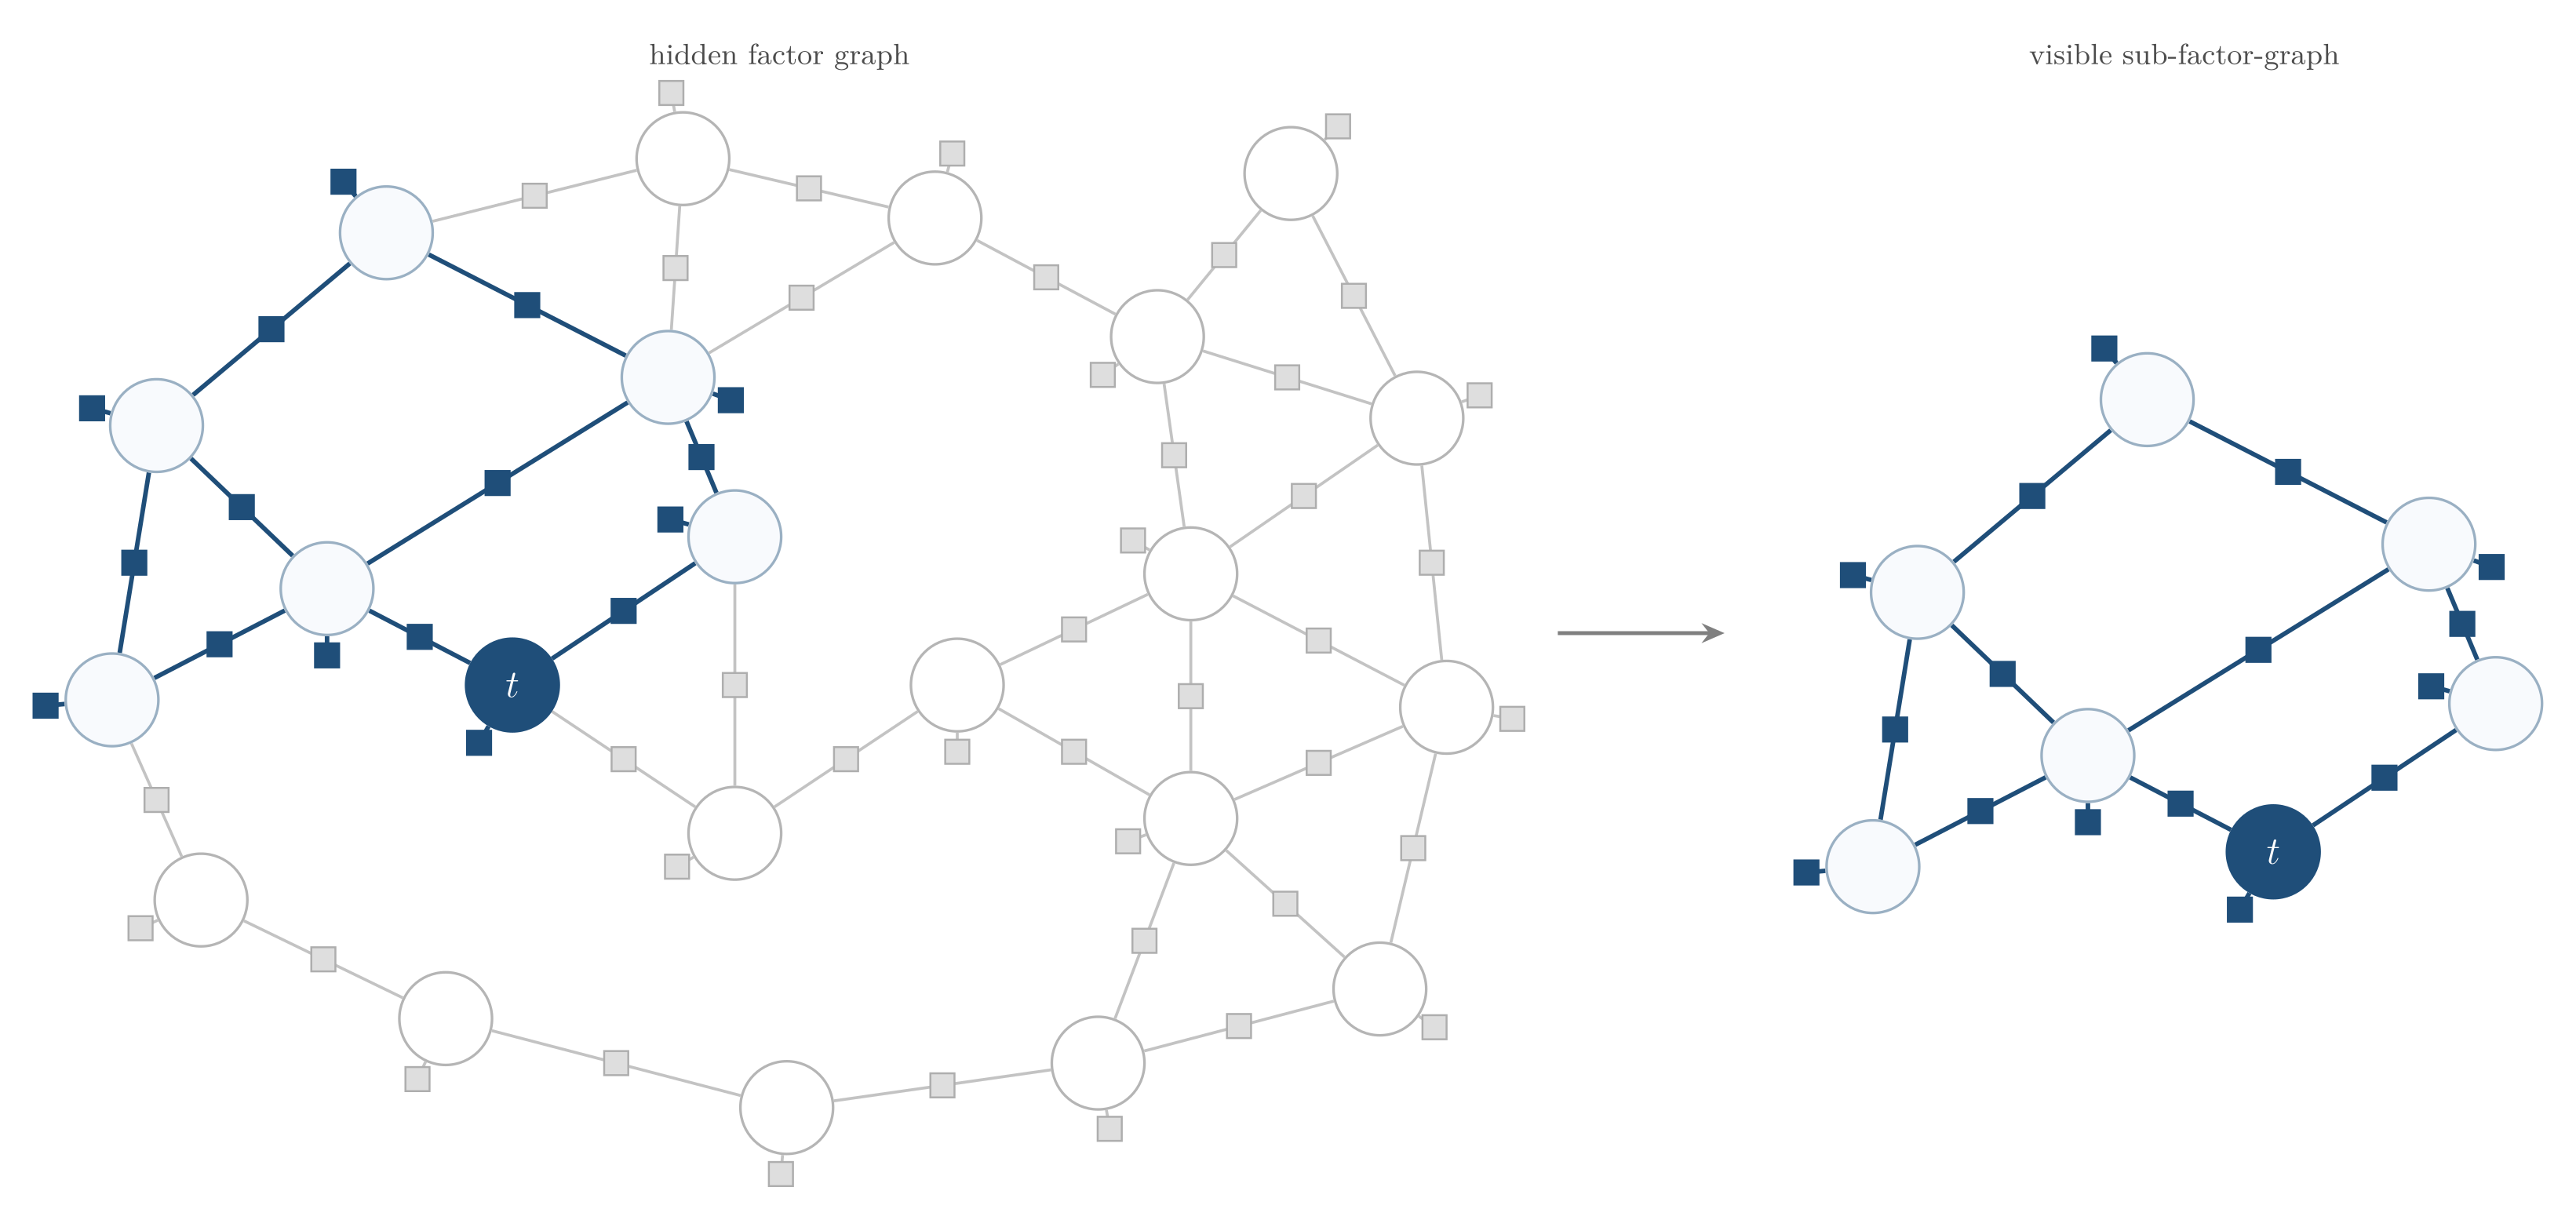
\includegraphics[width=.94\textwidth]{figures/images/01_transcript.png}
\caption{The hidden model and an induced transcript. Circles are variables;
squares are factors. A factor survives precisely when every variable it
touches has been revealed. The target $t$ is present from the beginning.}
\end{figure}

\subsection{The game and its error}
Both players know all tables and unary factors. Starting from $S=\{t\}$,
Max and Min alternate revealing a previously unrevealed non-target vertex,
with $h$ moves each. Max wants the final $L_S$ large and Min wants it small.
Assume $2h\le |V|-1$, so every move is legal. For Max first, backward
induction gives
\begin{equation}
 D_{S,0}=L_S,\qquad
 D_{S,\ell}=\begin{cases}
 \displaystyle\max_{v\notin S}D_{S\cup\{v\},\ell-1},&\ell>0\text{ even},\\[3pt]
 \displaystyle\min_{v\notin S}D_{S\cup\{v\},\ell-1},&\ell\text{ odd},
 \end{cases}\qquad D_{2h}=D_{\{t\},2h}.
 \label{eq:game}
\end{equation}
All our bounds also hold with Min first. The outcome is the value under
optimal play. They are not guarantees for arbitrary player strategies.
There is no penalty for computation and no option to change a revealed
factor. A disconnected component of $G[S]$ cancels from the ratio in
\eqref{eq:logit}; only the component containing $t$ affects the judge.

We measure error in natural-log odds, $\err$. If the desired metric is
probability, the sigmoid $s(x)=(1+e^{-x})^{-1}$ satisfies
\begin{equation}
 |s(x)-s(y)|\le\tanh\frac{|x-y|}{4}\le\frac{|x-y|}{4}.
 \label{eq:probability}
\end{equation}
For a fixed separation, its maximum occurs when $x$ and $y$ are symmetric
about zero, which proves the first inequality. Thus a logit error of $0.1$
implies a probability error below $0.025$. A large logit error need not
imply a large probability error when both logits are saturated.

There is no ground-truth assignment in the performance criterion.
Agreement with $L_V$ is agreement with the fully informed judge's model.
A misspecified full model can still be wrong about the world.

\clearpage
\section{Cores and oscillation}
\label{sec:cores}

\subsection{A set that settles the question}
A \emph{core} is a connected set $K\subseteq V$ containing $t$. Its
completion interval and its \emph{oscillation} are
\begin{equation}
 [a_K,b_K]=\left[\min_{K\subseteq S\subseteq V}L_S,
                     \max_{K\subseteq S\subseteq V}L_S\right],\qquad
 \osc(K)=b_K-a_K.
 \label{eq:osc}
\end{equation}
The tables stay fixed while $S$ varies. Completions can be disconnected,
and need not fit the debate budget. Enlarging $K$ shrinks the family of
completions, so it cannot increase the oscillation.

Suppose a core contains $100$ non-target vertices and every completion has
log-odds between $1.2$ and $1.3$. A player with $100$ moves can reveal the
whole core, counting any vertices the opponent reveals toward the same goal.
Max thereby guarantees at least $1.2$; Min guarantees at most $1.3$.
The full-model answer belongs to the same interval.

\begin{lemma}[Forcing a core]
\label{lem:forcing}
If $|K|\le h+1$, then
\begin{equation}
 a_K\le D_{2h}\le b_K,\qquad \err\le\osc(K).
 \label{eq:forcing}
\end{equation}
\end{lemma}
\begin{proof}
On each move, Max reveals a remaining non-target vertex of $K$, if one
exists, and otherwise makes any legal move. Every resulting terminal set
contains $K$, so the strategy guarantees $a_K$. The identical construction
for Min guarantees $b_K$. Finally $K\subseteq V$ implies $L_V\in[a_K,b_K]$.
\end{proof}

The two forcing strategies are considered separately. Neither needs to be
played at equilibrium. Connectivity was not used in the proof; it will let
us organize influence by paths. The bound can be minimized over cores
chosen after seeing the tables.

\begin{figure}[htbp]
\centering
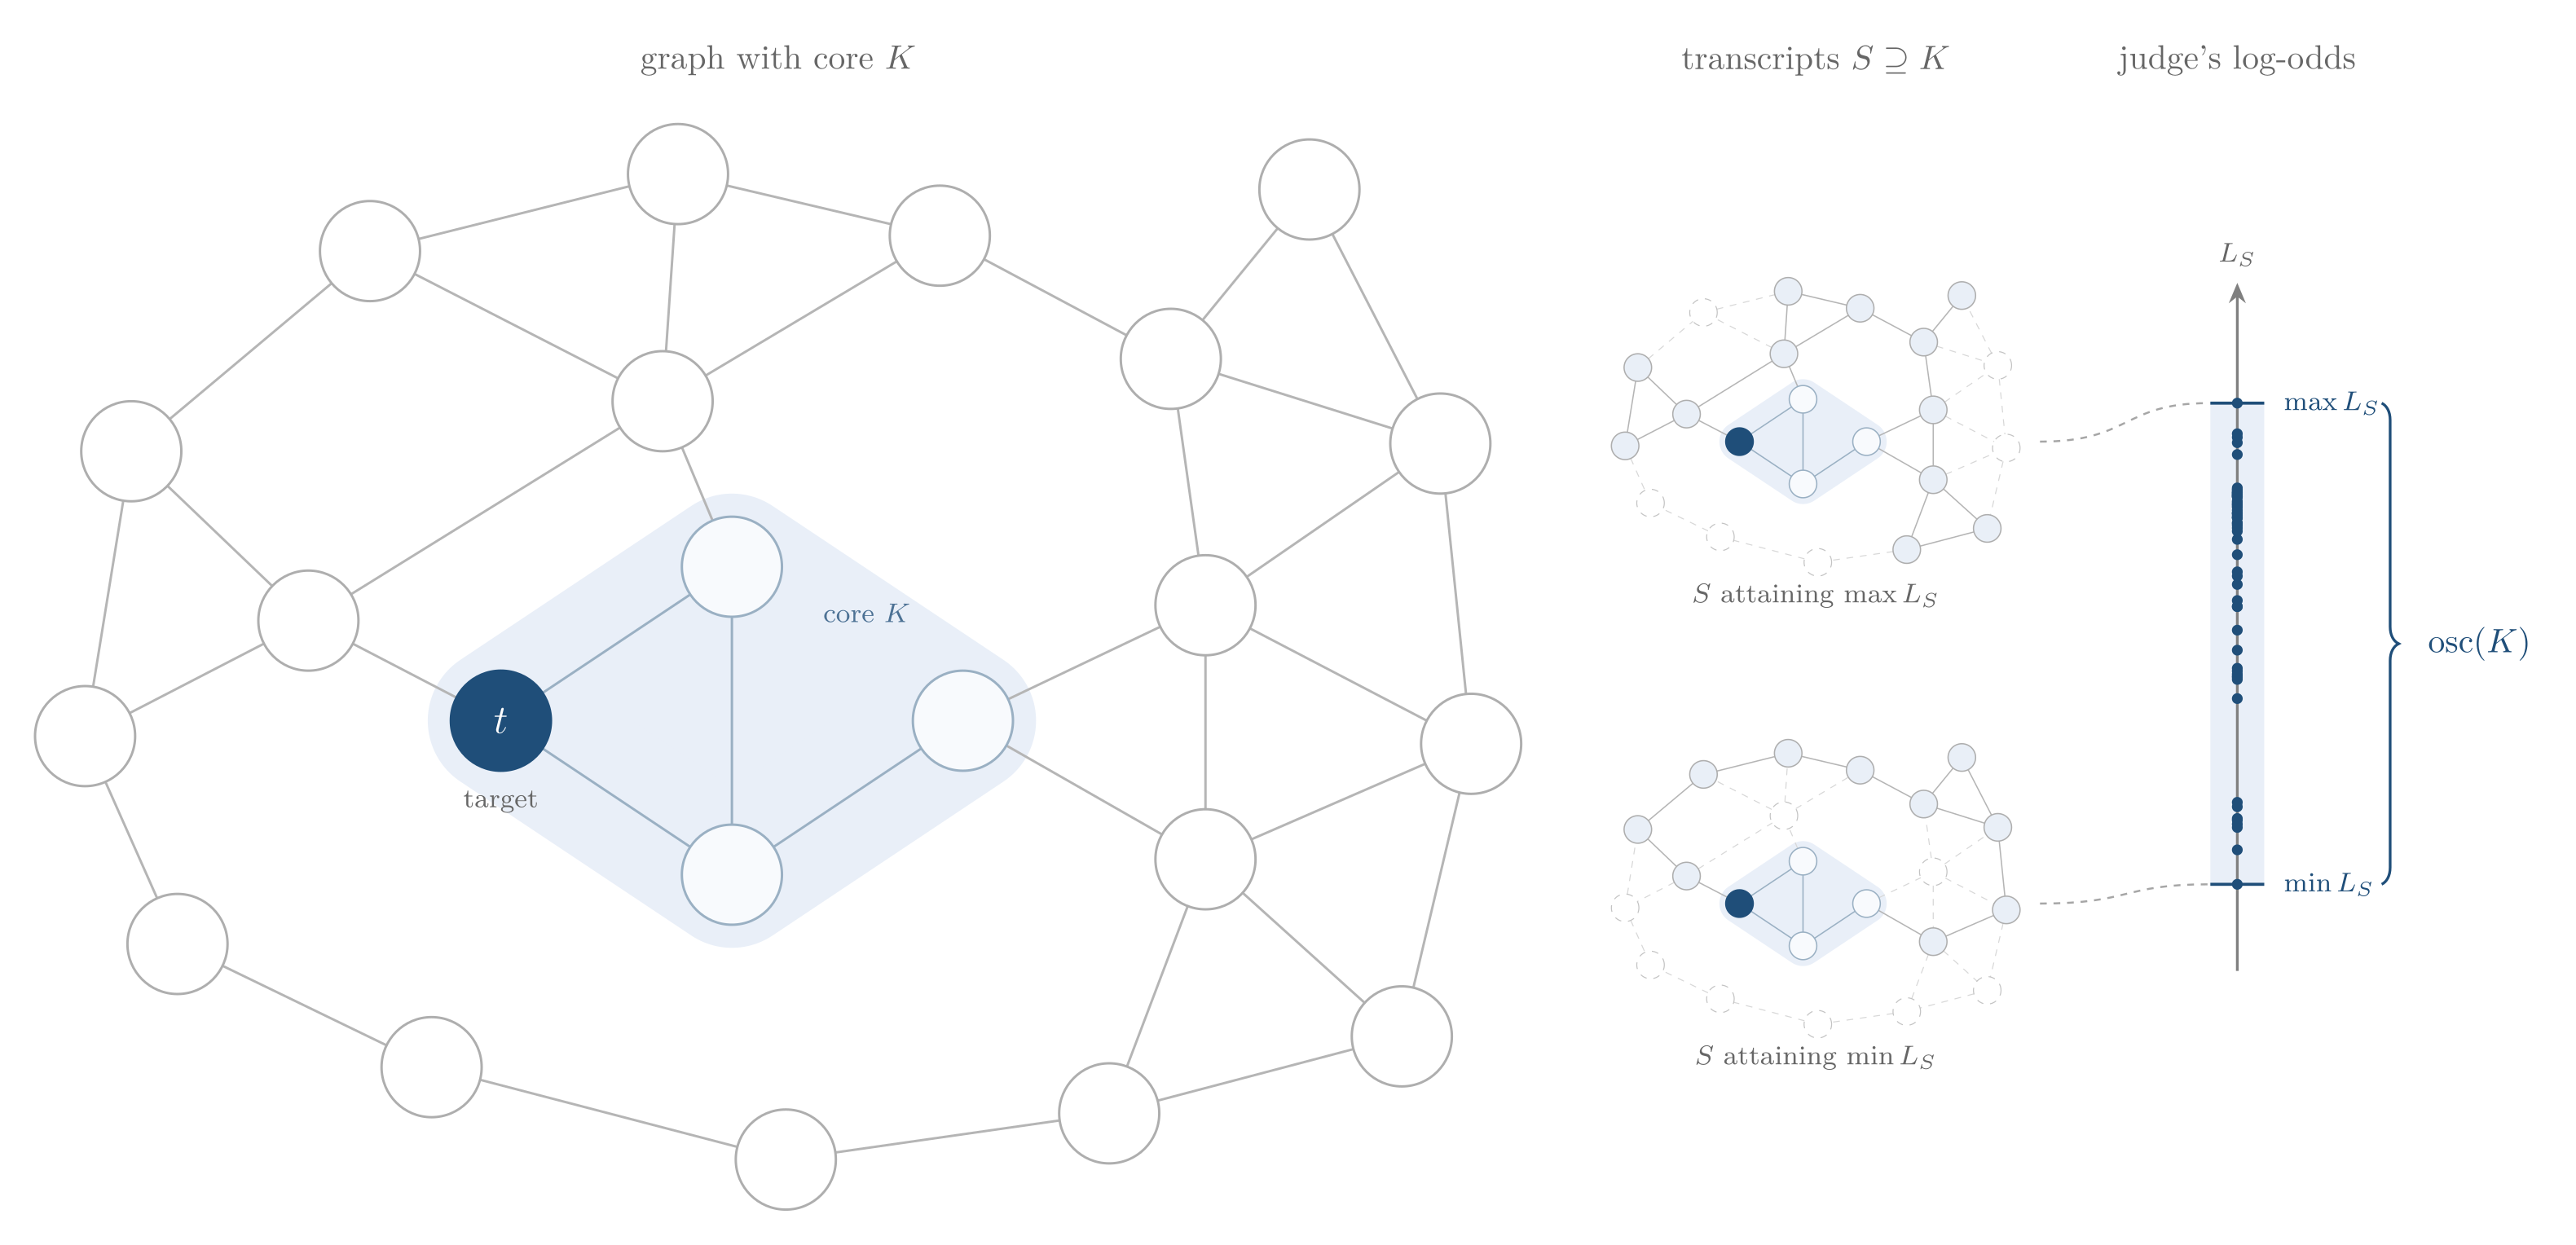
\includegraphics[width=.94\textwidth]{figures/images/02_core_oscillation.png}
\caption{Several transcripts containing a common core. Oscillation is the
full range over \emph{all} such completions, including the full graph. A few
pictured completions illustrate the definition without defining its extrema.}
\end{figure}

\subsection{What the first experiments measure}
For one board, let $O_h=\min_{|K|\le h+1}\osc(K)$, with the minimum over
connected cores containing $t$. Then $\err\le O_h$ board by board.
The curve $O_h$ is nonincreasing; the error of an alternating game need not
be. A first successful budget is therefore not a theorem of convergence at
every later budget.

\begin{figure}[htbp]
\centering
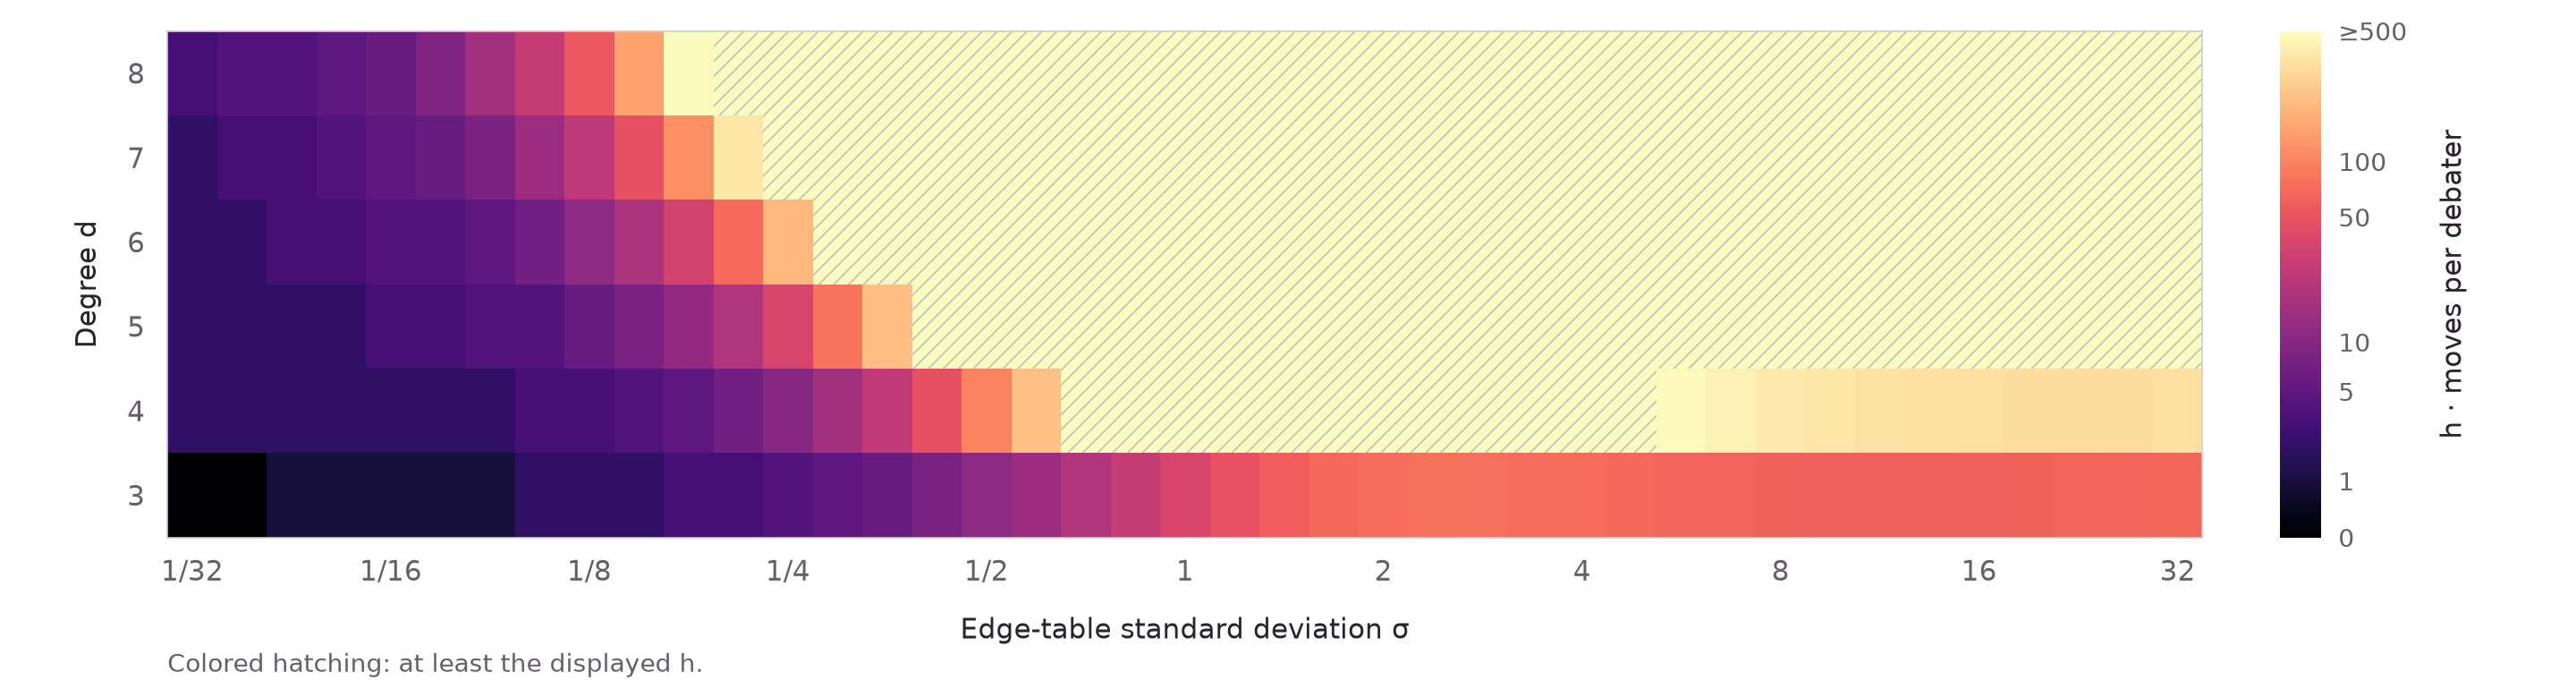
\includegraphics[width=.95\textwidth]{figures/images/03_core_mean.png}
\caption{A numerical crossing of the \emph{sample mean} of $O_h$ at $0.1$.
Each cell uses $1{,}000$ iid Gaussian-table draws on a $50{,}000$-vertex
partially filled regular tree, with zero unary factors. Colors use the upper
numerical crossing, capped at $500$. This is not the mean of the individual
boards' crossing budgets, and is not a population confidence guarantee.}
\label{fig:core}
\end{figure}
\begin{figure}[htbp]
\centering
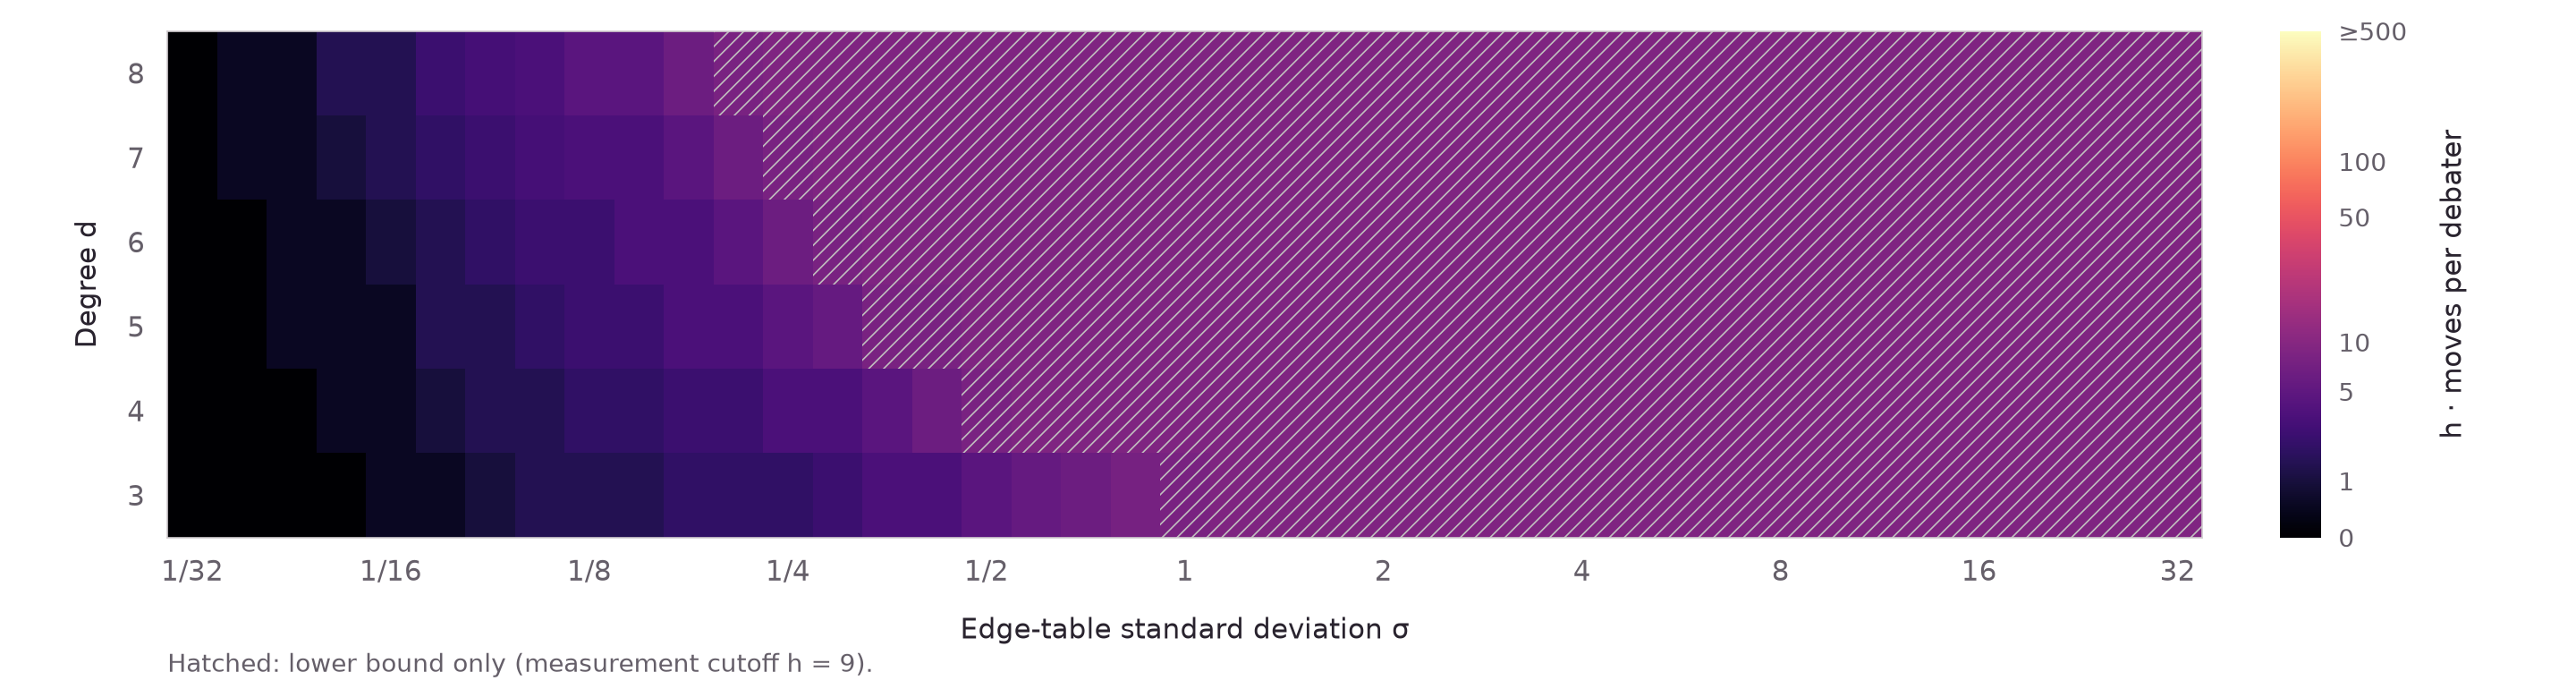
\includegraphics[width=.95\textwidth]{figures/images/04_alternating_debate.png}
\caption{The first budget at which mean absolute debate error is below
$0.1$, on the finite tree balls specified in the figure data. Colors summarize
statistical brackets; hatching marks lower bounds where success is
unresolved. Most hatched cells mean $h\ge9$, some boundary cells $h\ge8$.
The simultaneous $95\%$ statistical coverage is conditional on the guarded
floating-point strategy enclosures. The core and debate panels use different
tree sizes and sampling procedures, so a pixel comparison is not a paired
empirical test of \eqref{eq:forcing}.}
\end{figure}
\begin{figure}[htbp]
\centering
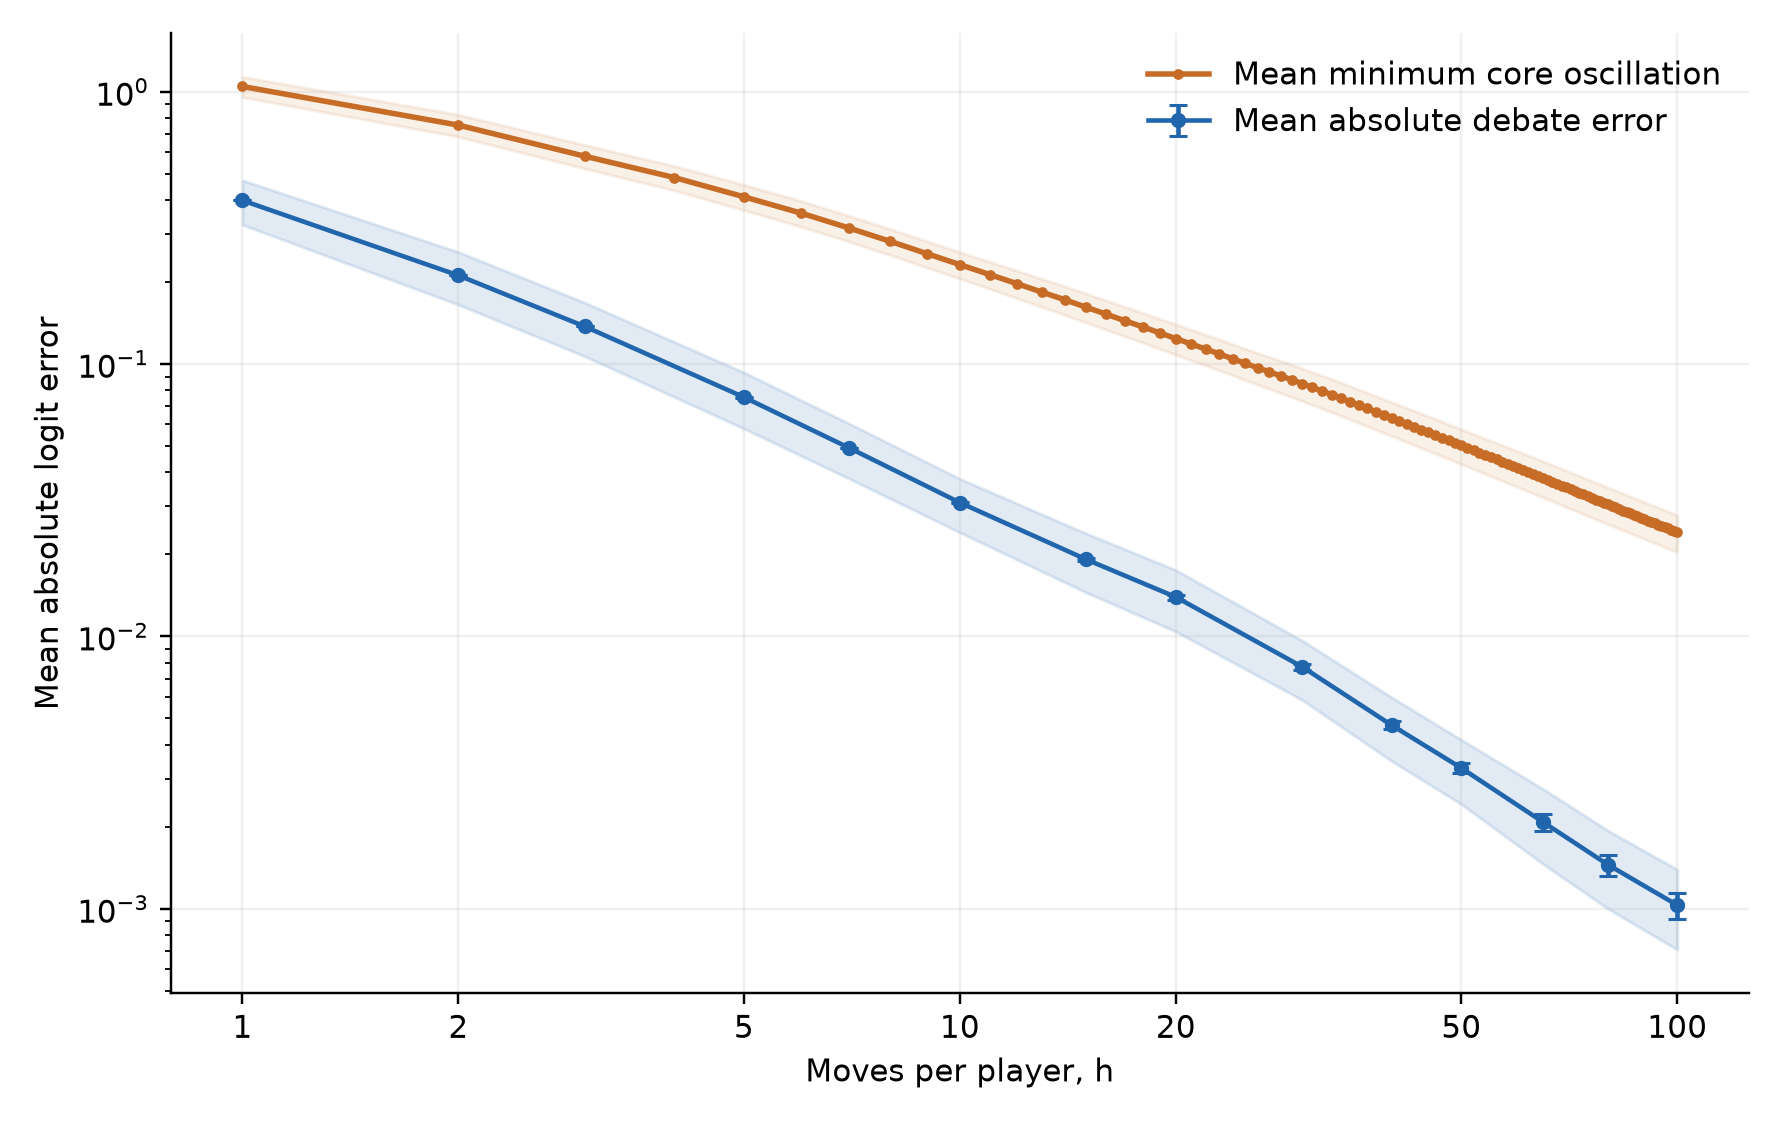
\includegraphics[width=.83\textwidth]{figures/images/05_debate_core.png}
\caption{A paired comparison: degree $4$, $\sigma=0.35$, zero unary factors,
and tree balls of depth $8$ ($13{,}121$ vertices). The $64$ draws use seeds
$7$--$70$. Blue is mean absolute debate error and orange is mean optimal-core
oscillation on those same boards. Bars represent numerical enclosures;
shading adds approximate pointwise $95\%$ sampling uncertainty. A roughly
straight segment on logarithmic axes suggests a power over the displayed
range, without identifying an asymptotic exponent.}
\label{fig:paired}
\end{figure}

\clearpage
\section{Factor-specific debate bounds}
\label{sec:factor}

\subsection{What one edge can transmit}
To understand a core's boundary, first consider a single edge $e=\{u,v\}$.
Every binary table has the expansion
\begin{equation}
 \theta_{(u,v)}(x_u,x_v)
 =a_e+\tfrac12 H_{e,u}x_u+\tfrac12 H_{e,v}x_v
                         +\tfrac12 J_e x_ux_v.
 \label{eq:contrast}
\end{equation}
For example,
\begin{align*}
 H_{e,u}&=\tfrac12(\theta_{++}+\theta_{+-}-\theta_{-+}-\theta_{--}),\\
 H_{e,v}&=\tfrac12(\theta_{++}-\theta_{+-}+\theta_{-+}-\theta_{--}),\\
 J_e&=\tfrac12(\theta_{++}-\theta_{+-}-\theta_{-+}+\theta_{--}).
\end{align*}
The constant $a_e$ cancels from odds. The two $H$'s are local fields
contributed by the edge; $J_e$ is its interaction. Our convention puts
$J_e/2$ in the energy, which accounts for the factors of two below.

On a tree, remove $e$ and let $z$ be the log-odds at $v$ on its side of
the cut. Summing over $x_v$ shows that the edge contributes to $u$ the message
\begin{equation}
 H_{e,u}+r_{J_e}(z+H_{e,v}),\qquad
 r_j(x)=\log\cosh\frac{x+j}{2}-\log\cosh\frac{x-j}{2}.
 \label{eq:message}
\end{equation}
For $j\ge0$, differentiation gives
\begin{equation}
 r_j'(x)=f_j(x)=\frac{\sinh j}{\cosh x+\cosh j},\qquad
 0\le f_j(x)\le f_j(0)=\tanh(j/2).
 \label{eq:slope}
\end{equation}
The response is odd in both $x$ and $j$, so for either sign of $j$ its
Lipschitz constant is $c_e=\tanh(|J_e|/2)$. It takes values between
$-|J_e|$ and $|J_e|$. Large $|x|$ makes its slope small: an already
strongly biased input has little remaining capacity to change the output.

An absent edge contributes zero. A present edge with its far endpoint
pinned contributes $H_{e,u}\pm J_e$. Therefore every possibility lies in
\[
 \reach_{(u,v)}=[\min(0,H_{e,u}-J_e,H_{e,u}+J_e),
                  \max(0,H_{e,u}-J_e,H_{e,u}+J_e)].
\]
Its width is
\begin{align}
 I_{(u,v)}
 &=|J_e|+\max(|H_{e,u}|,|J_e|)\notag\\
 &=\tfrac12|\theta_{(u,v)}(+,+)-\theta_{(u,v)}(-,+)|
  +\tfrac12|\theta_{(u,v)}(+,-)-\theta_{(u,v)}(-,-)|+|J_e|.
 \label{eq:reach}
\end{align}
This follows from the identity that the range of three numbers equals
half the sum of their three pairwise distances. $I$ is directed because
it measures the effect at a specified endpoint; $J$ and $c$ are not.

\subsection{Routes, gates, and cycles}
A route $P=(t,w_1,\ldots,w_r)$ is a self-avoiding path: no vertex appears
twice. Its length is $r$. The empty route consists of $t$ alone. A
\emph{core routing} $\routing$ is a set of routes contained in $K$, containing
the empty route and every prefix of each of its members. The routing need
not reach every vertex of $K$.

A \emph{gate} is a pair $(P,(v,u))$ where $P$ ends at $v$, $u$ is not on
$P$, and appending $u$ gives a route outside $\routing$. A gate may lead to
a vertex still inside $K$ if that extension was omitted from the routing.
A physical edge may occur at several gates, after different histories.
Cycle-closing steps are not gates.

\begin{figure}[htbp]
\centering
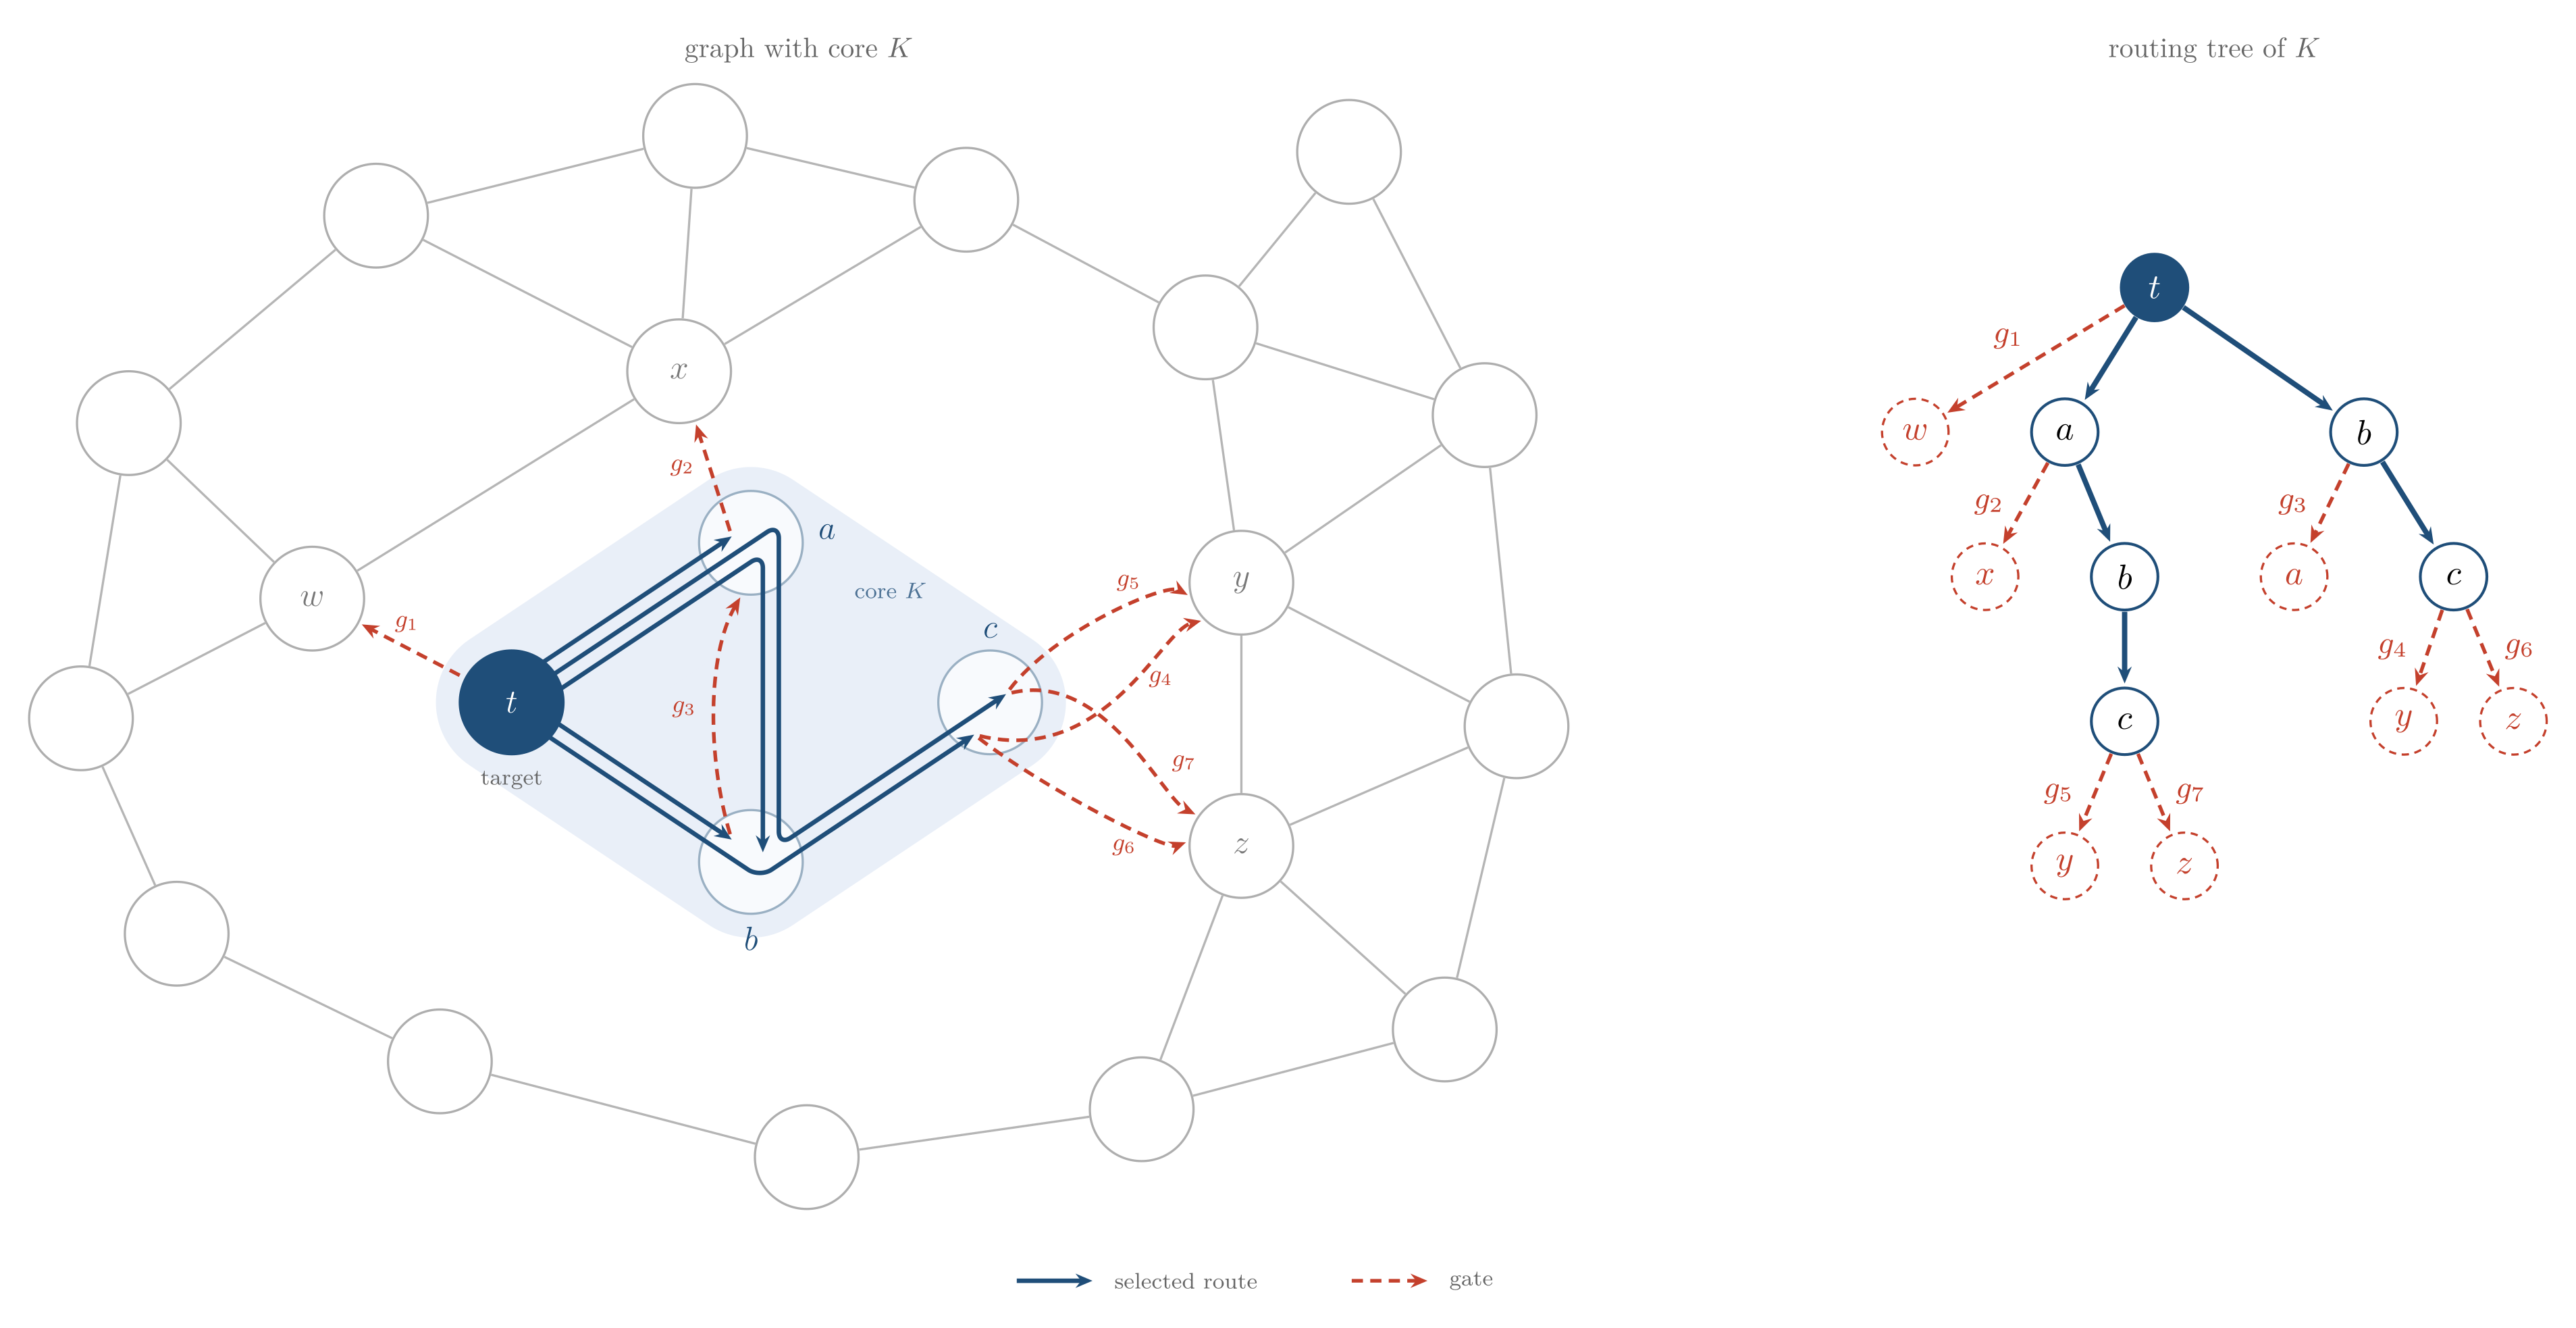
\includegraphics[width=.95\textwidth]{figures/images/06_core_routing.png}
\caption{A routing viewed on the graph and as a tree of path histories.
Different histories ending at the same physical vertex are different tree
states. Red dashed arrows are omitted self-avoiding extensions. In general
these include omitted internal extensions as well as exits from the core.}
\end{figure}

Here is why a tree of histories can represent a graph with cycles exactly.
Order the edges once and for all. To compute odds at $v$, first fix $x_v=-1$,
then switch its incident factors one at a time to their $x_v=+1$ versions.
The ratio of partition functions telescopes into one ratio per edge.
In the ratio for $\{v,u\}$, delete $v$; its other incident edges become unary
factors at their other endpoints, with $v$ pinned according to whether that
edge has already been switched. The remaining ratio is exactly the
one-edge calculation \eqref{eq:message}, using the cavity odds at $u$ in
that smaller model.

Repeat. Each ordinary recursive step deletes the previous vertex, so the
ordinary states are self-avoiding paths. A return to an earlier vertex is
replaced by its fixed pinned contribution. The recursion terminates because
the graph is finite. This is the binary self-avoiding-walk construction
associated with Weitz and its graphical-model extensions
\cite{weitz,jungshah}. The telescoping argument also shows why the same
edge order gives compatible pins in every induced submodel containing a
specified route. No independence of different history branches is asserted.

\subsection{From boundary intervals to an error certificate}
Truncate this recursion at the routing. Keep its internal messages and its
fixed cycle pins; at each gate allow an independent parameter throughout
$\reach_{(v,u)}$. Every completion $S\supseteq K$ supplies one permissible
choice of gate parameters: its true message if the extension is present,
zero if absent. Thus the root interval of the relaxed recursion contains
every $L_S$.

At an internal state, input widths add and the response multiplies their
sum by at most $c_e$ on the arrival edge. At the root, widths simply add.
Propagating from the leaves toward the root therefore proves the following
statement at the moment we have all its ingredients.

\begin{theorem}[Core routing certificate]
\label{thm:core}
For arbitrary finite tables and unary factors, every core $K$ and routing
$\routing$ satisfy
\begin{equation}
 \osc(K)\le\sum_{(P,e)\in\operatorname{gate}(\routing)}
                       I_e\prod_{e'\in P}\tanh(|J_{e'}|/2).
 \label{eq:routing}
\end{equation}
If $|K|\le h+1$, the same expression bounds $\err$.
\end{theorem}
\begin{proof}
Let $\Delta_P$ be a nonroot state's output width. Its input is the sum of
fixed terms, child messages, and gate parameters. Hence
\[
 \Delta_P\le c_{\mathrm{arrival}(P)}
 \left(\sum_{Q\text{ child of }P}\Delta_Q+
              \sum_{(P,e)\text{ gate}}I_e\right).
\]
The corresponding root inequality has no leading $c$. Expanding it
recursively gives exactly one summand per gate in \eqref{eq:routing}.
The completion containment just proved bounds $\osc(K)$ by this root width;
Lemma~\ref{lem:forcing} then bounds debate error.
\end{proof}

The gate edge contributes its reach, and is \emph{not} also included in the
product. Both the core and routing may depend on the realized tables.
Taking all self-avoiding routes inside $K$ leaves only gates exiting $K$.
On a tree this is one route to each core vertex. On a loopy graph a chosen
spanning tree alone does not suffice unless its omitted extensions are
also charged.

The interval construction is an upper bound, not a formula for exact
oscillation. For example, a single edge with $J\ne0$ but zero $H$'s and
unary fields has $L_{\{t\}}=L_V=0$. Its singleton core has oscillation zero,
whereas the relaxed reach has width $2|J|$.

\clearpage
\section{Ensemble bounds}
\label{sec:ensemble}

\subsection{Random fields help attenuate influence}
Now fix the graph and sample all four entries of each edge table
independently from $N(0,\sigma^2)$, independently across edges. The unary
factors are arbitrary and fixed. They may also be random with any joint law
independent of all edge tables, since we can condition on them first.
The three contrasts in \eqref{eq:contrast} are orthogonal. Consequently
$H_{e,u},H_{e,v},J_e$ are independent $N(0,\sigma^2)$ variables.

This observation is more useful than a bound on the largest table entry.
An input to a message contains several fresh Gaussian fields. Those fields
usually shift the input away from the location where the response has its
largest slope. Averaging the interval recursion exploits this shift.
Simply replacing each $c_e$ in \eqref{eq:routing} by its expectation would
give a different and weaker calculation.

Define
\begin{equation}
 g_\sigma=\frac{(2+\sqrt2)\sigma}{\sqrt\pi},\qquad
 \alpha_m(\sigma)=\E\frac{\sinh(\sigma|Z_0|)}
 {\cosh(\sqrt m\sigma Z_1)+\cosh(\sigma|Z_0|)},
 \label{eq:alpha}
\end{equation}
where $Z_0,Z_1$ are independent standard Gaussians and $m\ge1$.
The first quantity is the mean reach $\E I_e$: the two single differences
in \eqref{eq:reach} have variance $2\sigma^2$, and $J$ has variance
$\sigma^2$. The second quantity is the mean slope when the input contains
an independent Gaussian of variance $m\sigma^2$.

\begin{lemma}[Averaging an interval]
\label{lem:average}
Let $T\sim N(0,m\sigma^2)$, and let $j\ge0$. For every real $z$,
\[
 \E f_j(T+z)\le\E f_j(T)=:c_m(j).
\]
If an interval $[A,B]$ is independent of $T$, then, conditionally on $A,B,j$,
\[
 \E_T[r_j(T+B)-r_j(T+A)]\le c_m(j)(B-A).
\]
Also $\E_J c_m(|J|)=\alpha_m(\sigma)$ for $J\sim N(0,\sigma^2)$,
and $\alpha_m$ decreases with $m$.
\end{lemma}
\begin{proof}
The function $f_j$ is even and decreases with $|x|$. Expressing it as a
superposition of indicators of centered intervals reduces the first claim
to the fact that a centered Gaussian puts most mass in an interval of a
given length when that interval is centered at zero. Integrate this bound
between $A$ and $B$ to obtain the second claim. Increasing the variance
reduces the mass in each centered interval, proving the last assertion.
\end{proof}

We must check where the fresh Gaussian comes from, especially in a graph
with cycles. Fix a routing independently of the tables. At a state $P$
ending at $v$, let $m(P)$ be the number of incident edges that are
\emph{not} gate edges there. This includes the arrival edge, ordinary
children, and cycle pins. Their fields at $v$ sum to an independent
$N(0,m(P)\sigma^2)$ variable. Once these fields are removed, the remainder
of the input interval does not use them: a strict descendant cannot revisit
$v$. It also cannot reuse the arrival coupling, whose two endpoints are
already on the route. Gate fields are kept inside their gate intervals
and are not counted as fresh.

Apply Lemma~\ref{lem:average} to this input interval, then average the
independent arrival coupling. If $P$ has children $Q$ and $b_P$ gates,
\begin{equation}
 \E\Delta_P\le\alpha_{m(P)}(\sigma)
       \left(\sum_Q\E\Delta_Q+b_Pg_\sigma\right).
 \label{eq:mean-recursion}
\end{equation}
Different children can reuse physical variables. Only their individual
expectations are added in this equation; none are multiplied together.
Unrolling gives
\begin{equation}
 \E\osc(K)\le g_\sigma
 \sum_{(P,e)\in\operatorname{gate}(\routing)}
       \prod_{\substack{\emptyset\ne P'\preceq P}}
                      \alpha_{m(P')}(\sigma).
 \label{eq:mean-routing}
\end{equation}
Unlike the deterministic bound, this averaged formula assumes the routing
was fixed without looking at the tables. Substituting a data-dependent
optimal routing would invalidate the fresh-variable argument.

\subsection{A radius becomes a budget}
For $d\ge3$, put $q=d-1$ and define
\begin{equation}
 \rho=\rho(d,\sigma)=\max_{2\le m\le d}(m-1)\alpha_m(\sigma).
 \label{eq:rho}
\end{equation}
An intermediate vertex of physical degree $m$ has at most $m-1$
self-avoiding continuations and average attenuation $\alpha_m$.
Their combined cost is therefore at most $\rho$. The maximum over $m$
is what makes the argument uniform over graphs with nonconstant degree.

The ball $B_R(t)$ contains at most
\[
 1+d\sum_{j=0}^{R-1}q^j=1+d\frac{q^R-1}{d-2}
\]
vertices. Therefore the affordable radius is
\begin{equation}
 R_h=\left\lfloor\frac{\log(1+(d-2)h/d)}{\log q}\right\rfloor.
 \label{eq:radius}
\end{equation}
Use the routing of all paths of length at most $R_h$. Its gates occur
at depth $R_h$. The last state has at most $q$ gates and at least one
fresh field, so it costs at most $q\alpha_1g_\sigma$. Every earlier
nonroot generation multiplies the sum by at most $\rho$, while the root
has at most $d$ branches.

\begin{theorem}[Gaussian mean-error bound]
\label{thm:upper}
Let $G$ have maximum degree at most $d\ge3$, and let $h\ge1$ with
$2h\le |V|-1$. If $\rho(d,\sigma)<1$, set
\[
 \gamma=\frac{\log(1/\rho)}{\log(d-1)},\qquad
 C(d,\sigma)=\alpha_1(\sigma)g_\sigma
       \frac{d(d-1)}{\rho^2}\left(\frac d{d-2}\right)^\gamma.
\]
Then, uniformly in graph size, target, and fixed unary factors,
\begin{equation}
 \boxed{\E\err\le C(d,\sigma)h^{-\gamma}.}
 \label{eq:upper}
\end{equation}
For $R_h\ge1$ a sharper finite-budget version is
\[
 \E\err\le d g_\sigma\min\{1,q\alpha_1\rho^{R_h-1}\};
\]
for $R_h=0$, use $d g_\sigma$.
\end{theorem}
\begin{proof}
The preceding path count and \eqref{eq:mean-routing} give the second bound;
the singleton core gives $d g_\sigma$. Since
$R_h-1\ge\log_q(1+(d-2)h/d)-2$, the path count for $R_h\ge1$ gives
\[
 \rho^{R_h-1}\le\rho^{-2}(1+(d-2)h/d)^{-\gamma}
                  \le\rho^{-2}(d/(d-2))^\gamma h^{-\gamma}.
\]
When $R_h=0$, $h<d$. To check the same constant, let $m$ maximize $\rho$.
Then $\rho=(m-1)\alpha_m\le q\alpha_1$, and
\[
 \frac{C h^{-\gamma}}{d g_\sigma}
 \ge\rho^{-1}(d/((d-2)h))^\gamma
 =\left(\frac{qd}{(d-2)h}\right)^\gamma>1.
\]
Thus the stated power also covers small budgets.
\end{proof}

The hypothesis $\rho<1$ is essential to the \emph{decaying} power-law
statement. When it fails, it is the certificate that fails; this argument
has not established nonlocality or nonconvergence.

There is a useful all-scale conclusion at degrees three and four. The
identity $r_j'=f_j$ also gives
\[
 f_j(x)=\frac12\left(\tanh\frac{x+j}{2}-\tanh\frac{x-j}{2}\right).
\]
If $\Lambda$ has logistic distribution function
$(1+e^{-x})^{-1}$, this implies
\[
 \alpha_m(\sigma)=
 \Prob\bigl(|\sqrt m Z_1-\Lambda/\sigma|\le |Z_0|\bigr).
\]
For any fixed value of $|Z_0|$, adding an independent shift to the centered
Gaussian cannot increase its mass in that centered interval. Hence
\begin{equation}
 \alpha_m(\sigma)<a_m:=\Prob(\sqrt m|Z_1|\le|Z_0|)
          =\frac2\pi\arctan\frac1{\sqrt m},
 \label{eq:allscale}
\end{equation}
with equality in the limit $\sigma\to\infty$. The last expression follows
from the angular measure of the corresponding wedges in the plane.
The function $(m-1)a_m$ increases with $m$; differentiating
$(x-1)\arctan(x^{-1/2})$ verifies this. Therefore
\[
 \rho(3,\sigma)<\frac23,\qquad
 \rho(4,\sigma)<\frac6\pi\arctan\frac12<0.886.
\]
The mean-error theorem holds at every finite scale for these degrees.
At any fixed degree it also holds for sufficiently small $\sigma$, since
$\alpha_m(\sigma)\to0$ as $\sigma\downarrow0$.

\begin{figure}[htbp]
\centering
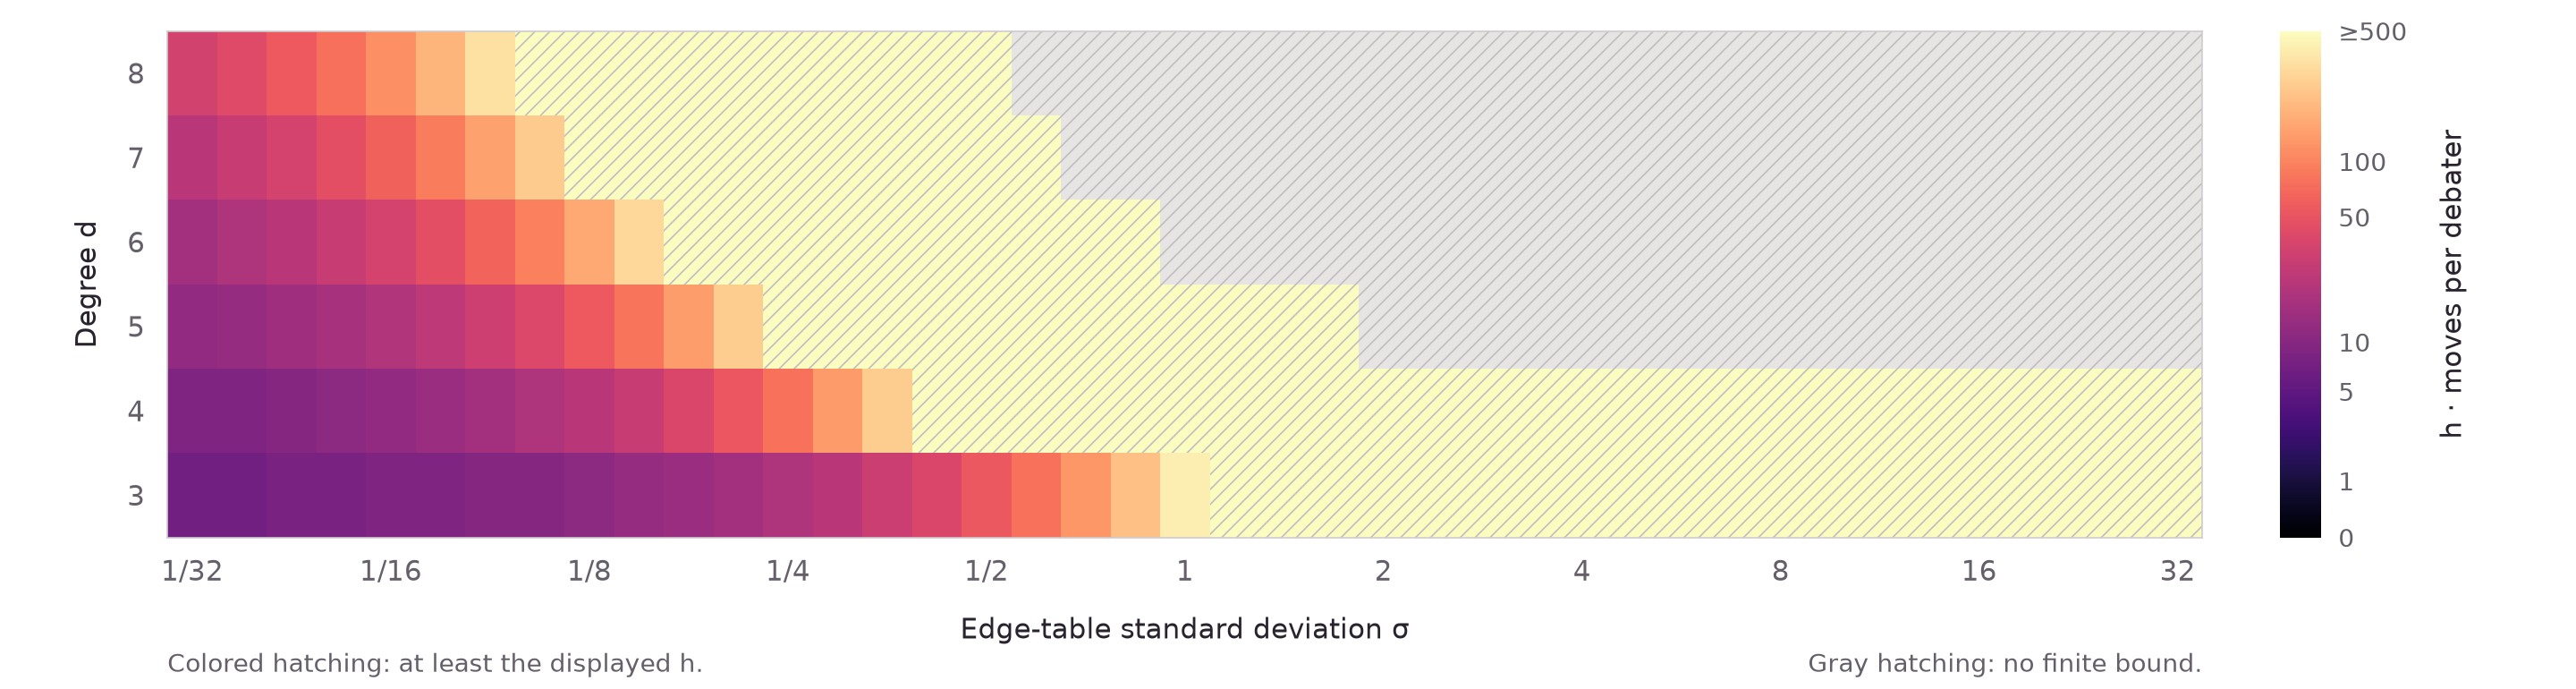
\includegraphics[width=.95\textwidth]{figures/images/07_ensemble_bound.png}
\caption{The smallest integer $h\ge1$ for which \eqref{eq:upper} is at most
$0.1$, evaluated by numerical quadrature. Colored hatching means a sufficient
budget at least $500$; gray hatching means $\rho\ge1$, so this formula supplies
no decaying guarantee. The calculation is uniform over all graph sizes; it
is not a simulation on a particular tree.}
\end{figure}
\begin{figure}[htbp]
\centering
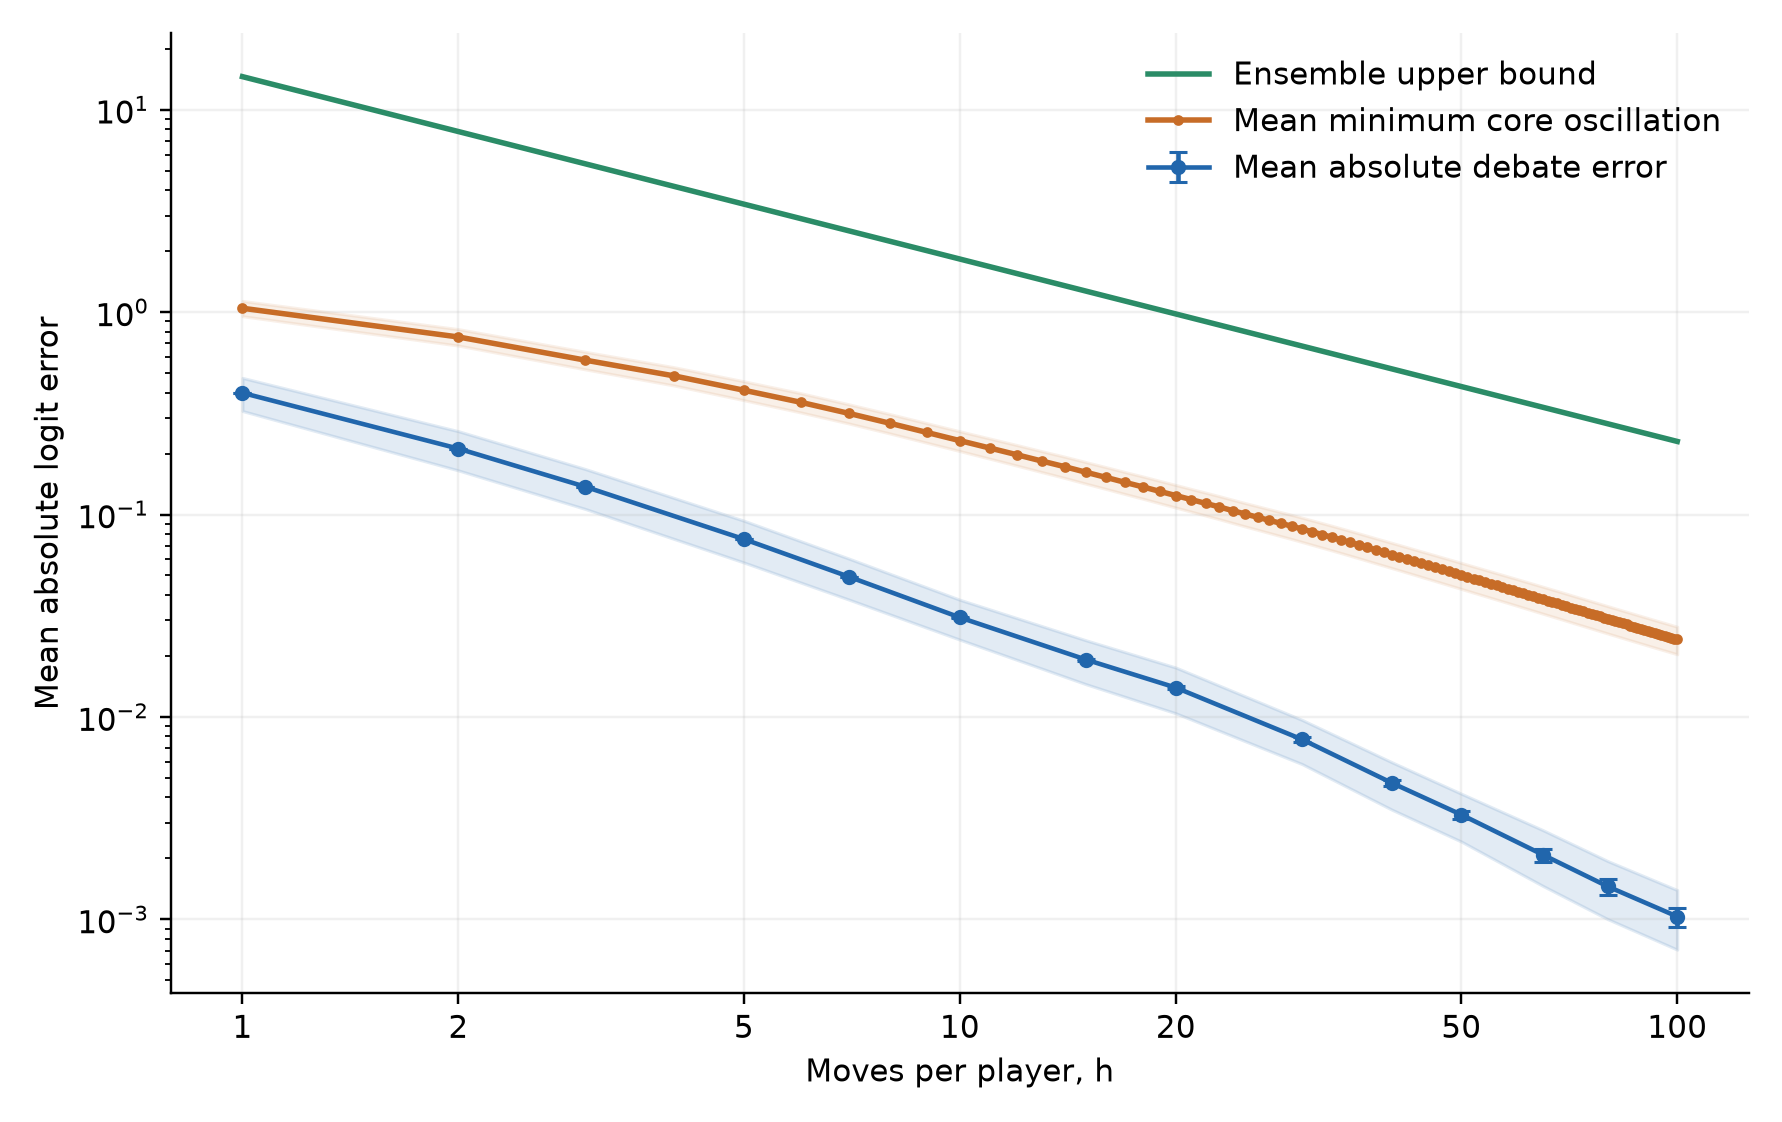
\includegraphics[width=.83\textwidth]{figures/images/08_debate_upper.png}
\caption{The paired experiment of Figure~\ref{fig:paired}, with the uniform
ensemble bound $14.57957h^{-0.9013297}$ added. Its constant and exponent are
calculated from the theorem without fitting to the data. Similar-looking
slopes over this budget range do not establish equal asymptotic exponents.}
\end{figure}

\subsection{High noise: what a fractional moment says}
\label{sec:highnoise}
The mean-error argument sees some saturation, but it does not exploit all
of it. A stronger calculation at large $\sigma$ controls
\[
 \|D_{2h}-L_V\|_p=(\E\err^p)^{1/p},\qquad 0<p<1.
\]
For such $p$ this is a quasi-norm. It gives less weight to rare large errors
than the mean does. Appendix~\ref{app:fractional} proves a fully explicit
bound $\|D_{2h}-L_V\|_p\le U(d,\sigma,h,p)$, valid on \emph{every} graph
of maximum degree three or four, including graphs with arbitrary cycles.
It yields, for any specified failure probability $\eta\in(0,1)$,
\begin{equation}
 \Prob\bigl(\err>\eta^{-1/p}U(d,\sigma,h,p)\bigr)\le\eta.
 \label{eq:confidence}
\end{equation}
At degree three, for example, $\sigma>6$ and $p=6/\sigma$ give a
fixed-confidence threshold
\[O_{\sigma,\eta}(h^{-\sigma\log(5/4)/(6\log2)}).\]
The exponent improves with $\sigma$, but the constants can be large.
Changing $p$ also changes the error metric; fixed confidence is the common
criterion in this comparison.

This does not establish a corresponding improvement of the mean-error
exponent. It does not establish a heavy-tailed error distribution either.
In fact there is a Gaussian tail envelope. If
$A_e=\theta_{(t,u)}(+,-)-\theta_{(t,u)}(-,-)$ and
$B_e=\theta_{(t,u)}(+,+)-\theta_{(t,u)}(-,+)$, then
\begin{equation}
 \err\le W:=\sum_{e\ni t}\bigl[\max(0,A_e,B_e)-\min(0,A_e,B_e)\bigr].
 \label{eq:envelope}
\end{equation}
Each summand is the maximum of
$A_e,-A_e,B_e,-B_e,A_e-B_e,B_e-A_e$. Thus $W$ is the maximum of at most
$6^d$ centered Gaussian linear forms, each of variance at most
$4d\sigma^2$. A Gaussian Chernoff bound and a union bound give
\begin{equation}
 \Prob(\err>u)\le\min\{1,6^d e^{-u^2/(8d\sigma^2)}\},\qquad u>0.
 \label{eq:tail}
\end{equation}
All moments exist at fixed $d,\sigma$. Rare errors can still matter for
estimating a mean; the tail's mathematical class is a separate issue.

\clearpage
\section{Lower bounds}
\label{sec:lower}

\subsection{Why an inspection budget leaves information behind}
An upper bound supplies a strategy. A lower bound must allow the players
to choose their strategy after seeing the entire board. Treating omitted
vertices as an independent random sample would miss that difficulty.

Work now on a regular degree-$d$ tree ball of depth $L$, with zero unary
factors. The root has $d$ children; every other nonleaf has $q=d-1$
children. All edge-table entries are independent $N(0,\sigma^2)$.
At depth $n+1$ there are $dq^n$ edges. We will build an orthonormal family
of random test functions, one per edge on that level. The full-model answer
correlates with all of them. A budgeted judge has a bound on the \emph{sum}
of its correlations, even though its selected transcript depends on all
the tables. The deficit gives an RMS error by orthogonal projection.

The distinction between a fixed tree and a family of trees matters. A
fixed finite model can eventually be fully revealed. A polynomial lower
bound as $h$ grows will therefore require a depth growing with $\log h$.
We will state that depth explicitly.

\subsection{Tests adapted to a path}
Orient messages toward the root, writing the edge message as
\[
 m_e=M_e+r_{J_e}(X_e),\qquad
 X_e=U_e+\sum_{f\text{ child of }e}m_f.
\]
$M_e$ is the field at the parent endpoint, $U_e$ the field at the child;
all $M_e,U_e,J_e$ are independent $N(0,\sigma^2)$ variables.
Let $c_e=\tanh(|J_e|/2)$. For an edge $e$ at depth $n+1$, write $f\prec e$
for its $n$ strict ancestor edges.

To include alternating game values without making false claims about
arbitrary selection rules, let $\Vcl_k$ be the class generated by terminal
logits whose target components contain at most $k$ non-target vertices,
using finite pointwise minima, maxima, and \emph{fixed} convex combinations.
All finite perfect-information reveal games with total budget $k$ lie in
this class, as do fixed averages of their values. Arbitrary discontinuous
board-dependent selections, or convex weights depending on the board, are
not automatically included.

Choose a nonnegative bounded function $w(J)$ with $\E w(J)^2=1$, and define
\[
 \Psi_e=\frac{M_e}{\sigma}\prod_{f\prec e}\sgn(J_f)w(J_f),\quad
 A_n=\E\prod_{f\prec e}|m_f'(X_f)|w(J_f),\quad
 C_e=\prod_{f\prec e}c_fw(J_f).
\]
Here $m_f'(X_f)$ means $r_{J_f}'(X_f)$. The number $A_n$ is the same for
every edge on the level by symmetry. If $c_fw(J_f)\le K$ always, then
$C_e\le K^n$.

\begin{lemma}[A budgeted projection]
\label{lem:projection}
For every $\mathsf V\in\Vcl_k$,
\begin{equation}
 \|\mathsf V-L_V\|_2\ge\frac{\sigma}{\sqrt{dq^n}}
                         (dq^n A_n-kK^n)_+.
 \label{eq:projection}
\end{equation}
Here and below $x_+=\max(x,0)$.
\end{lemma}
\begin{proof}
The $\Psi_e$ have norm one. For two different edges on the same level,
one factor $M_e$ is centered and independent of every other factor in the
product, so their inner product is zero. Hence they are orthonormal.
Gaussian integration by parts in $M_e$ gives
\[
 \langle L_V,\Psi_e\rangle
 =\sigma\E\left[\frac{\partial L_V}{\partial M_e}
             \prod_{f\prec e}\sgn(J_f)w(J_f)\right]=\sigma A_n.
\]
The chain rule supplied the product of actual slopes; the sign factors
make it nonnegative.

For a fixed terminal transcript the derivative is zero unless the edge
belongs to its target component, and otherwise is a product of the slopes
along its path. At most $k$ level edges can contribute. After multiplication
by the sign and weight factors, every contribution is between zero and
$K^n$. Finite minima, maxima, and fixed convex combinations are Lipschitz
in the Gaussian fields. Almost everywhere their gradients are convex
combinations of terminal gradients. The same pointwise bound on the sum
therefore survives, and integration by parts gives
\[
 0\le\sum_e\langle\mathsf V,\Psi_e\rangle\le\sigma kK^n.
\]
The sum of the full-model coefficients is $\sigma dq^n A_n$.
Bessel's inequality followed by Cauchy--Schwarz over the $dq^n$ coefficients
proves \eqref{eq:projection}.
\end{proof}

\subsection{A scalar inequality that survives the whole path}
Normalize fields by $\sigma$, and set
\begin{align}
 c(z)&=\tanh(\sigma|z|/2),\notag\\
 r(z,x)&=\frac2\sigma\artanh\left(\tanh\frac{\sigma z}{2}
                                      \tanh\frac{\sigma x}{2}\right),\notag\\
 \psi(z,x)&=\frac{1+\cosh(\sigma z)}{\cosh(\sigma x)+\cosh(\sigma z)}.
 \label{eq:normalized}
\end{align}
$\sigma r$ is the response, and $\psi$ is its actual slope divided by the
largest possible slope $c(z)$. The response is symmetric in law, because
changing the sign of $J$ changes its sign. Also $|r(z,x)|\le|z|$, so its
second moment is at most one.

Let $f:\R\to[0,1]$ be even, with $0<N:=\E[f(Z)^2/c(Z)^2]<\infty$.
Our choices below make the quotient bounded. Put
\[
 K=N^{-1/2},\qquad w(J)=K\frac{f(J/\sigma)}{c(J/\sigma)}.
\]
Then $\E w^2=1$ and $cw\le K$. The actual weighted slope on a path is
$Kf(Z)\psi(Z,X)$.

We need to average products of these slopes even though successive cavity
inputs are dependent. The following inequality does that work. Put
$\tau=d+2/\sigma^2$. For every $z,x$,
\begin{equation}
 \psi(z,x)e^{-r(z,x)^2/(2\tau)}\ge e^{-\sigma^2x^2/4}.
 \label{eq:carrier}
\end{equation}
To verify it, let $C=\cosh(\sigma z)$, $t=\cosh(\sigma x)$, and
$D=(1+Ct)/(t+C)^2$. Direct differentiation gives
\[
 (\log\psi)_{xx}=-\sigma^2D,\quad
 r_x^2=\frac{C^2-1}{(t+C)^2},\quad rr_{xx}\le0,\quad 2D+r_x^2\le1.
\]
Since $1/\tau\le\sigma^2/2$, the logarithm on the left of
\eqref{eq:carrier} has second derivative at least $-\sigma^2/2$.
It is even and equals zero at the origin. Integrating this derivative
bound twice proves the inequality.

Let $Y$ be the response on the continuing child edge. Conditional on its
subtree and its coupling, the normalized input one step nearer the root is
\[
 \sqrt d\,G+S+Y,
\]
where $G$ is standard Gaussian and $S$ is the sum of the other $q-1$
child responses. These quantities and the current coupling $Z$ are
independent; $S$ is symmetric and $\E S^2\le q-1$. Gaussian integration in
\eqref{eq:carrier} gives
\[
 \E_{Z,G}\bigl[f(Z)\psi(Z,\sqrt dG+x)
                   e^{-r(Z,\sqrt dG+x)^2/(2\tau)}\bigr]
 \ge\frac{\E f(Z)}{\sqrt{1+d\sigma^2/2}}e^{-x^2/(2\tau)}.
\]
Furthermore, symmetry and Jensen's inequality imply
\begin{align*}
 \E e^{-(S+y)^2/(2\tau)}
 &=e^{-y^2/(2\tau)}\E[e^{-S^2/(2\tau)}\cosh(Sy/\tau)]\\
 &\ge e^{-y^2/(2\tau)}e^{-(q-1)/(2\tau)}.
\end{align*}
Thus if
\begin{equation}
 \lambda=\frac{\E f(Z)}{\sqrt{1+d\sigma^2/2}}
              e^{-(q-1)/(2\tau)},\qquad v=e^{-1/(2\tau)},
 \label{eq:simple-lambda}
\end{equation}
conditional averaging of one step sends the auxiliary function
$e^{-y^2/(2\tau)}$ to at least $\lambda$ times itself. Iterate from the
root down the path. At its last response, Jensen gives an expectation at
least $v$. Since the auxiliary function is at most one, we have proved
\begin{equation}
 A_n\ge v(K\lambda)^n.
 \label{eq:path-gain}
\end{equation}
The auxiliary Gaussian is what keeps the dependence along the path under
control. Factoring the actual gains into independent one-edge expectations
would not be justified.

\subsection{The post's explicit lower bound}
All the ingredients are now in place. The next statement is deliberately
shorter to calculate than the stronger certificates in
Appendix~\ref{app:stronger}.

\begin{theorem}[An explicit RMS lower bound]
\label{thm:lower}
Let $d\ge3$, $\sigma>0$, and $q=d-1$. Define
\[
 A_0=\frac{q\exp(-(d-2)\sigma^2/(4+2d\sigma^2))}
                   {\sqrt{1+d\sigma^2/2}}.
\]
Suppose $A_0>1$. Set
\begin{align*}
 \varepsilon&=\tanh\left(\frac\sigma4(1-A_0^{-1})\right),\qquad
 C(Z)=\tanh(\sigma|Z|/2),\qquad
 F(Z)=\min\{1,C(Z)^2/\varepsilon^2\},\\
 a&=A_0\E F(Z),\qquad
 N=\E\frac{F(Z)^2}{C(Z)^2},\qquad
 \delta=\frac{\log(qN)}{2\log a}-1,
\end{align*}
with $Z$ standard Gaussian and the ratio defining $N$ continued by zero
at $Z=0$. Then $a>1$ and $\delta>0$.
For every integer $h\ge1$, on the Gaussian regular tree ball described
above with
\begin{equation}
 L\ge1+\left\lceil\frac{\log(2h)}{\log a}\right\rceil,
 \label{eq:lower-depth}
\end{equation}
and legal budget $2h\le |V|-1$, ordinary alternating debate satisfies
\begin{equation}
 \boxed{(\E\err^2)^{1/2}\ge
 \sigma\left(\sqrt d\,e^{-1/(2d)}-\frac1{\sqrt d}\right)(2ah)^{-\delta}.}
 \label{eq:lower}
\end{equation}
The same bound holds for every value in $\Vcl_{2h}$.
\end{theorem}
\begin{proof}
Put $u=(1-A_0^{-1})/2$. The event $C(Z)<\varepsilon$ is $|Z|<u$.
The density of $|Z|$ is less than one, so
$1-\E F\le u$ and $a\ge(A_0+1)/2>1$.
The quotient in $N$ is bounded by $\varepsilon^{-2}$. Cauchy--Schwarz and
$\E C^2\le\sigma^2/4$ imply
\[
 \frac{a^2}{qN}
 \le\frac{A_0^2}{q}\E C^2
 \le\frac{q\sigma^2}{4+2d\sigma^2}<\frac12.
\]
Consequently $\delta>0$ and $a/\sqrt{qN}=a^{-\delta}$.

Use $f=F$ in \eqref{eq:simple-lambda}. Then $q\lambda=a$.
Substituting \eqref{eq:path-gain} in Lemma~\ref{lem:projection} gives,
for every available level $n+1$,
\begin{equation}
 \|D_{2h}-L_V\|_2\ge
 \sigma\sqrt d\,v\,a^{-\delta n}
            \left(1-\frac{2h}{dv a^n}\right)_+.
 \label{eq:finite-lower}
\end{equation}
Choose $n=\lceil\log_a(2h)\rceil$, which is allowed by
\eqref{eq:lower-depth}. Then $a^n\ge2h$, and
$a^{-\delta n}\ge(2ah)^{-\delta}$. Since $\tau\ge d$,
$\sqrt d\,v-1/\sqrt d\ge\sqrt d\,e^{-1/(2d)}-1/\sqrt d>0$.
This proves the result.
\end{proof}

The square on $\varepsilon$ in $F$ matters: it makes the threshold
$C<\varepsilon$, which is exactly the small-ball estimate used in the
proof. The theorem gives a lower bound on RMS, while the preceding
ensemble theorem bounded mean absolute error. Those are different metrics.
An RMS lower bound alone does not imply an equally large mean lower bound.
Appendix~\ref{app:lone} performs a separate tail conversion.

\begin{figure}[htbp]
\centering
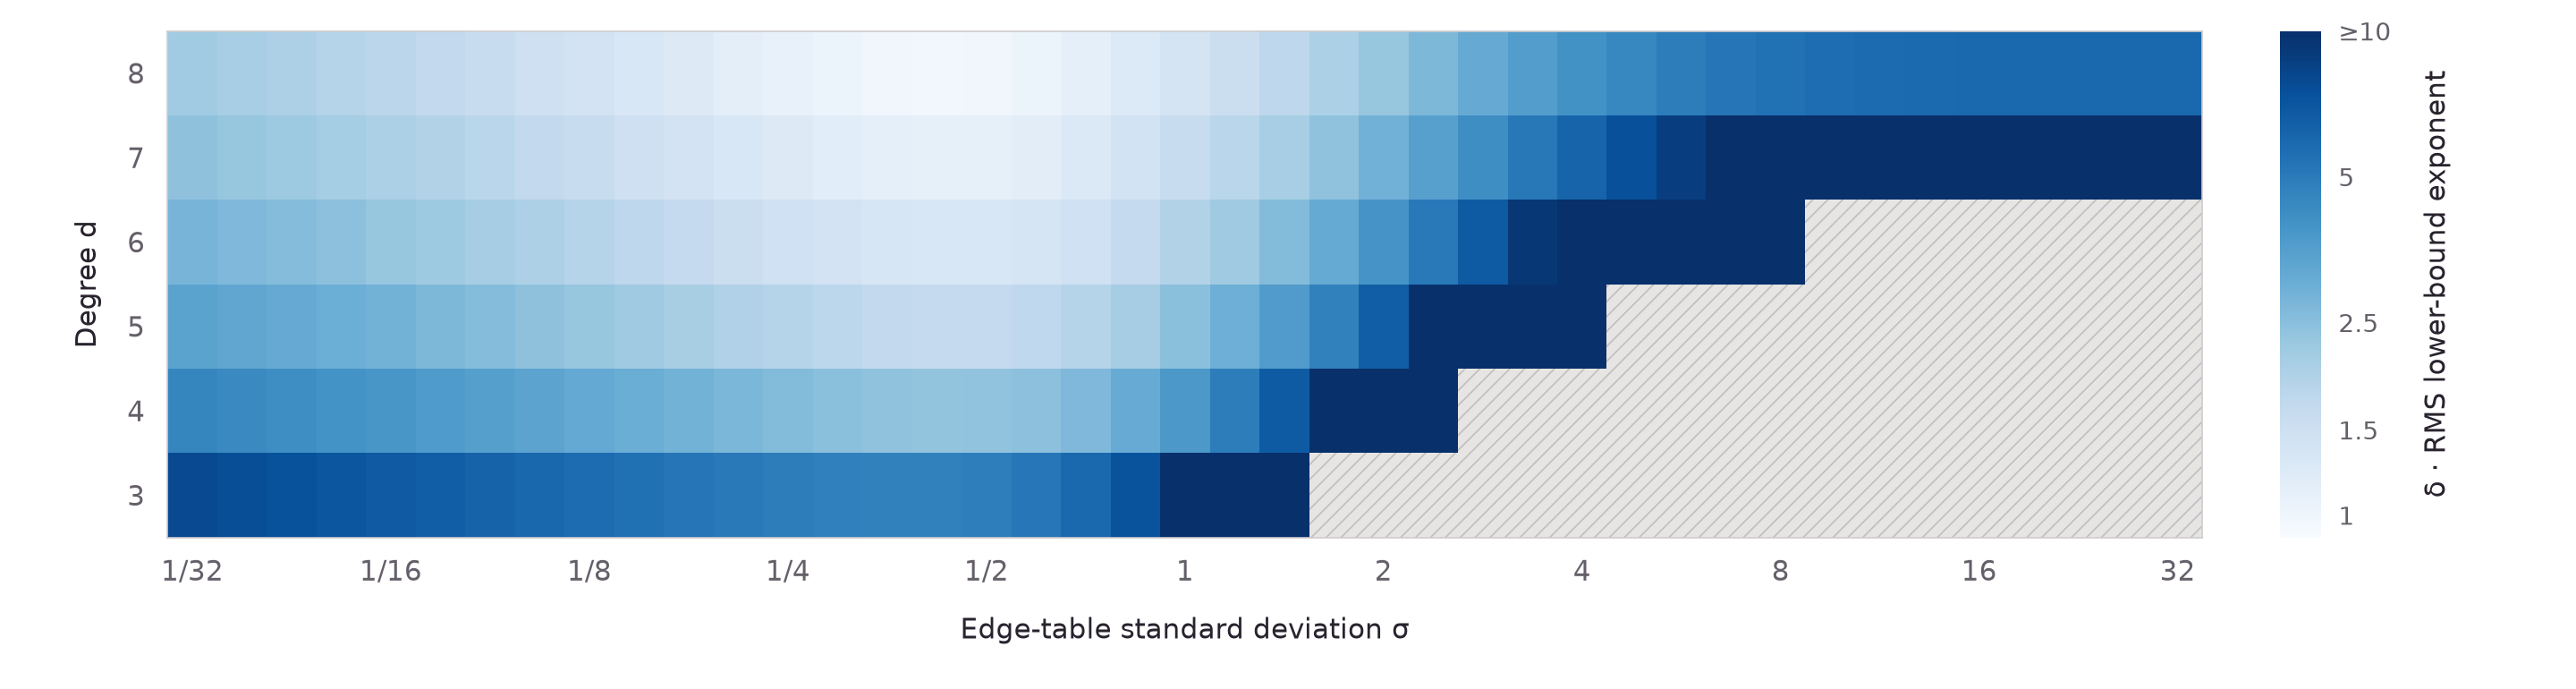
\includegraphics[width=.95\textwidth]{figures/images/09_lower_exponents.png}
\caption{RMS lower-bound exponents from the stronger certificate family
in Appendix~\ref{app:stronger}. The $193$ populated cells are numerical
quadrature evaluations, not outward-certified decimal inequalities or
optimal exponents. Smaller $\delta$ means slower decay and a stronger
asymptotic obstruction; prefactors and required depth still matter. Hatched cells
fail the condition $A_0>1$ of Theorem~\ref{thm:lower} and were not evaluated
with the stronger certificates; this does not show that polynomial lower
bounds are impossible there.}
\end{figure}
\begin{figure}[htbp]
\centering
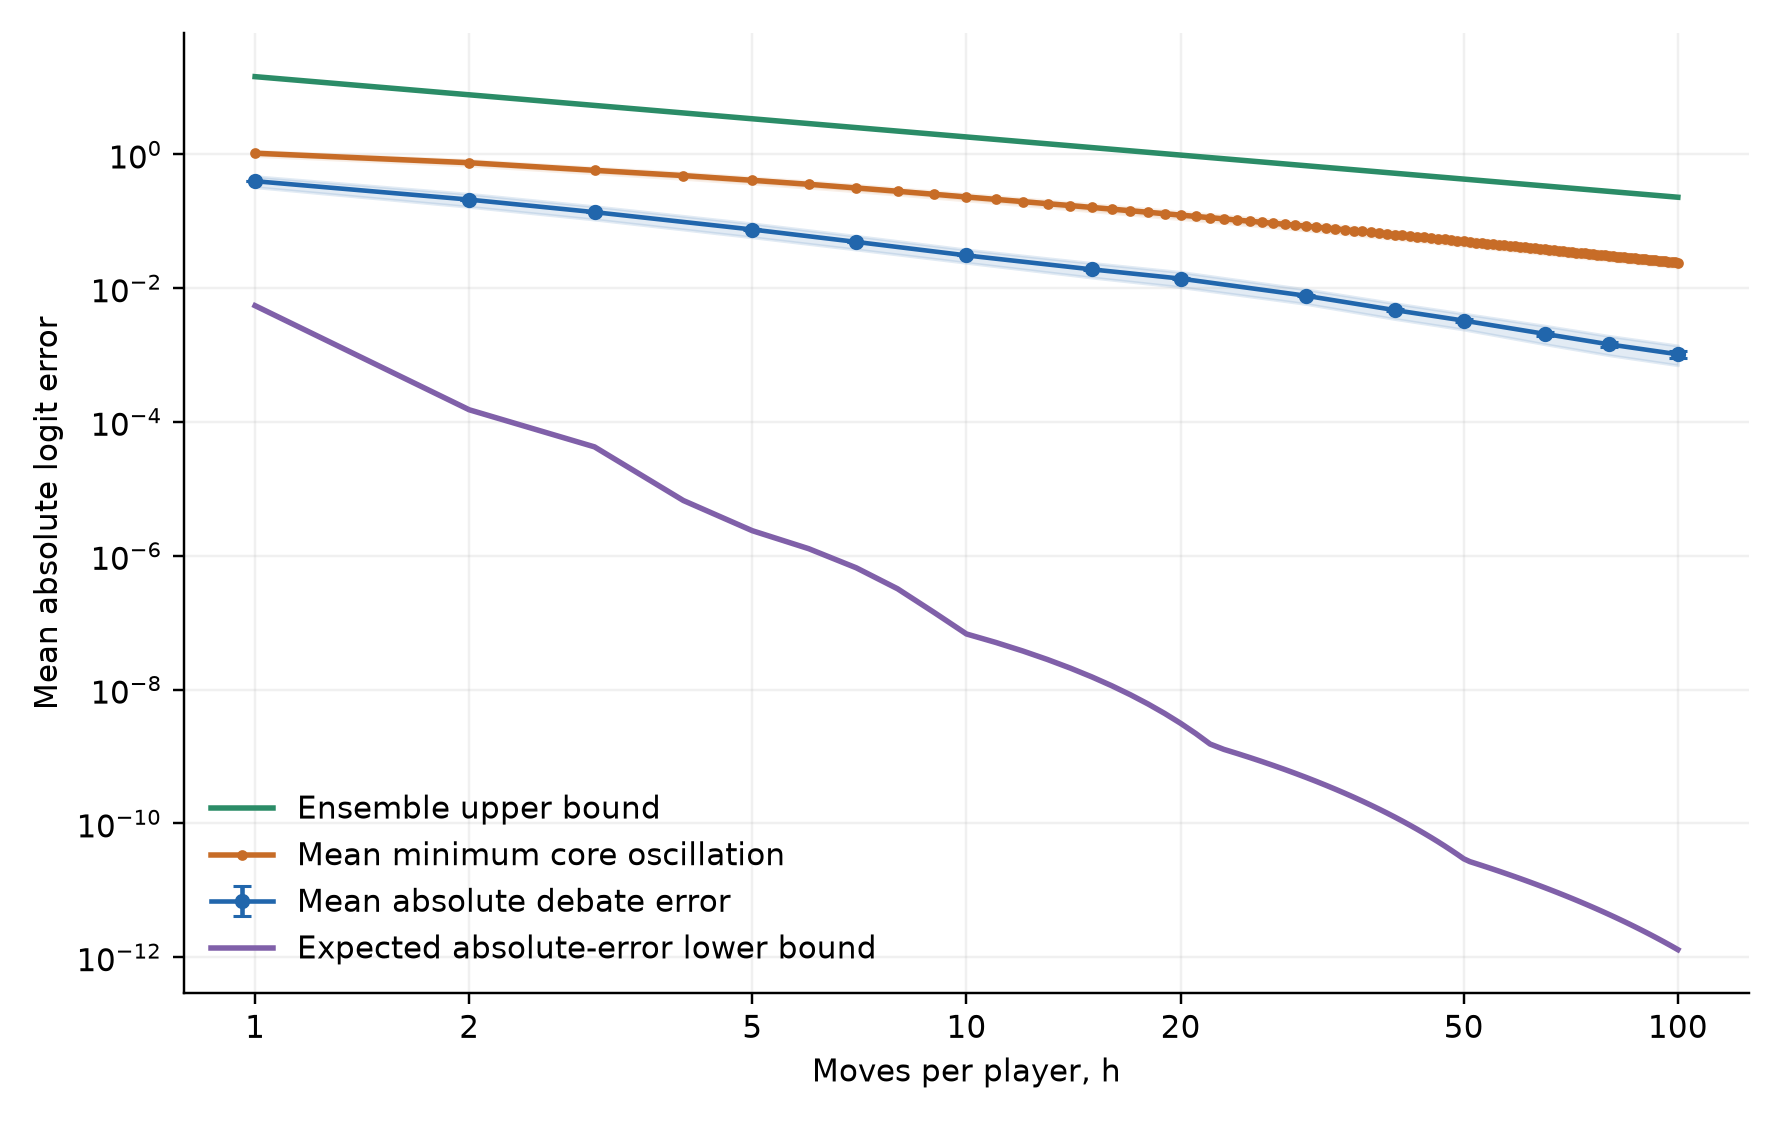
\includegraphics[width=.83\textwidth]{figures/images/10_debate_bounds.png}
\caption{The same finite-depth experiment as Figure~\ref{fig:paired}, now
with a population \emph{mean absolute-error} lower bound in purple.
It is obtained by optimizing \eqref{eq:finite-lower} over the eight available
levels using stronger constants, then applying the tail conversion
\eqref{eq:lone}. At $h=1,10,100$ its values are approximately $0.00550$,
$6.79\cdot10^{-8}$, and $1.30\cdot10^{-12}$. It is neither an RMS curve
nor a confidence limit for the empirical mean. The quadrature is numerical,
without outward rounding.}
\end{figure}

\clearpage
\section{Next steps and the limits of the conclusion}

The forcing argument is insensitive to the order of the players' moves;
what it uses is that either player can fit a useful core into its own quota.
The hard part is estimating how stable a small core can be. Random fields,
weak edges, and cancellations can make a particular core far better than a
uniform radius bound predicts.

A different protocol could ask for intermediate numerical claims and allow
a challenge to descend a single branch. Such a protocol would need a rule
for what is asserted, what is checked, and how errors propagate. It would
also change the judge. The lower bound here concerns the induced-submodel
judge and the class $\Vcl_k$; it is not an impossibility theorem for recursive
verification or debate in general.

Likewise, the failure of a particular contraction criterion leaves an open
mathematical question. Neither a gray heatmap cell nor a run stopped at a
budget cutoff proves a nonlocal regime. Extending useful bounds into these
regions requires an argument that keeps the actual model and error metric
in view. Results about additive or affine tree games cannot be transferred
to nonlinear factor-graph messages without such an argument.

Finally, an agreement theorem for an idealized judge addresses only one
part of supervision. Applying the model to programming, politics, or
philosophy would require evidence that the chosen variables, factorization,
revelation rule, and local computation describe the task. Those applications
motivate the question; the mathematics here does not classify those domains.

\appendix
\clearpage
\section{An explicit high-noise fractional-moment bound}
\label{app:fractional}

This appendix supplies the quantitative statement used in
Section~\ref{sec:highnoise}. Its proof uses marginal moments of interval
widths, so cycles introduce no independence assumption between siblings.

\begin{theorem}[Fractional moment and confidence]
\label{thm:fractional}
Under the assumptions of Theorem~\ref{thm:upper}, let $d\in\{3,4\}$ and
$h\ge d$. Choose $p$ in the indicated interval:
\[
\begin{array}{c|ccc}
 d&\bar\rho_d&b_d&\text{allowed }p\\\hline
 3&2/3&4/5&12/(5\sigma)<p<1\\
 4&89/100&27/25&108/(11\sigma)<p<1
\end{array}
\]
Put $n=R_h-1\ge0$, with $R_h$ as in \eqref{eq:radius}, and
\[
 \lambda=\bar\rho_d+\frac{b_d}{\sigma p},\qquad
 \mu=\bar\rho_d^{1-p/3},\qquad
 S_n=\sum_{j=0}^{n-1}\lambda^{n-1-j}\mu^j.
\]
The sum is zero for $n=0$. For $n\ge1$ it equals
$(\lambda^n-\mu^n)/(\lambda-\mu)$ when $\lambda\ne\mu$, and
$n\lambda^{n-1}$ when $\lambda=\mu$. Then
\begin{equation}
 \|D_{2h}-L_V\|_p\le U(d,\sigma,h,p)
 :=\sigma\left\{d\left[\frac85\lambda^n+
                  \frac32(d-1)^2 S_n\right]\right\}^{1/p}.
 \label{eq:fractional}
\end{equation}
The confidence statement \eqref{eq:confidence} follows for every
$\eta\in(0,1)$.
\end{theorem}

\begin{proof}
Normalize fields and logits by $\sigma$. A coupling $j\sim N(0,1)$ has
normalized response $r(j,x)$ as in \eqref{eq:normalized}, with absolute slope
\[
 F_{\sigma,j}(x)=\frac{\sinh(\sigma|j|)}
                       {\cosh(\sigma x)+\cosh(\sigma|j|)}
 \le e^{-\sigma(|x|-|j|)_+}.
\]
Truncate the walk recursion at depth $R_h$. At each terminal state allow
its cavity input to range over all real numbers. Its response interval
has width $W_0=2|j|$. At an interior state, let $W_r$ denote the output
width after $r$ layers have been propagated. Always $W_r\le2|j|$.

Suppose the state has $k$ ordinary children and physical degree $m$.
Then $k\le m-1\le q$. Conditional on all child intervals and cycle-pin
shifts, their input is a fixed interval $I$ of length
$u=\sum_{i=1}^k W_{r,i}$, translated by a fresh $T\sim N(0,m)$.
The arrival coupling $j$ is also fresh. This is precisely the local
independence established before \eqref{eq:mean-recursion}. When $k=0$
the width is zero. Otherwise $m\ge2$ and
\[
 W_{r+1}\le u\sup_{x\in T+I}F_{\sigma,j}(x).
\]
By Lemma~\ref{lem:average} and \eqref{eq:allscale},
$\E[W_{r+1}\mid I]\le a_m u$.

For an even decreasing function $g:\R\to[0,1]$, allowing its argument to
range over an interval of length $u$ enlarges each superlevel interval by
$u$. The Gaussian density is at most $1/\sqrt{2\pi m}$, and translations
of a centered interval only reduce its mass. Layer-cake integration gives
\[
 \E_T\sup_{x\in T+I}g(x)\le\E_Tg(T)+\frac{u}{\sqrt{2\pi m}}.
\]
Use $g=F_{\sigma,j}^p$ and average $j$. If
$A_m(c)=\E e^{-c(\sqrt m|Z_1|-|Z_0|)_+}$, this yields
\begin{equation}
 \E[W_{r+1}^p\mid I]\le
 u^p\left(A_m(\sigma p)+\frac{u}{\sqrt{2\pi m}}\right).
 \label{eq:frac-step}
\end{equation}
The positive part of $\sqrt m|Z_1|-|Z_0|$ has density on $x>0$
\[
 g_m(x)=\sqrt{\frac8{\pi(m+1)}}e^{-x^2/(2(m+1))}
       \Phi_{\mathrm N}\left(-\frac{x}{\sqrt{m(m+1)}}\right),
\]
where $\Phi_{\mathrm N}$ is the standard Gaussian distribution function.
Both factors decrease for $x>0$. Its density is therefore at most
$g_m(0)=\sqrt{2/(\pi(m+1))}$, so
\[
 A_m(c)\le a_m+\frac1c\sqrt{\frac2{\pi(m+1)}}.
\]
The tabulated constants satisfy, for $1\le k\le q$,
\[
 k a_{k+1}\le\bar\rho_d,\qquad
 k\sqrt{\frac2{\pi(k+2)}}\le b_d.
\]
Both left sides increase with $k$. For $d=3$ use $a_3=1/3$ and
$\sqrt{2/\pi}<4/5$; for $d=4$ use
$3a_4<89/100$ and $3\sqrt{2/(5\pi)}<27/25$.
These inequalities follow, for example, from $\pi>157/50$ and the
alternating series for $\arctan(1/2)$.
Thus $k A_m(\sigma p)\le\lambda<1$.

Let $w=\E W_0=\sqrt{8/\pi}<8/5$. Induction on mean widths and the
pointwise bound $W_r\le2|j|$ give
\[
 \E W_r\le w\bar\rho_d^r,\qquad \E W_r^4\le48.
\]
H\"older interpolation, with $1+p=(1-p/3)\cdot1+(p/3)\cdot4$, gives
\[
 \E W_r^{1+p}\le(\E W_r)^{1-p/3}(\E W_r^4)^{p/3}
                   \le5\mu^r.
\]
Let $y_r$ bound all $p$-moments at level $r$ uniformly over states and
graphs. Since $u^p\le\sum_iW_{r,i}^p$ and
$u^{1+p}\le k^p\sum_iW_{r,i}^{1+p}$, \eqref{eq:frac-step} implies
\[
 y_{r+1}\le\lambda y_r+\tfrac32q^2\mu^r,
 \qquad y_0\le w^p\le8/5.
\]
We used $1/\sqrt{2\pi m}<3/10$ and $k^{1+p}\le q^2$.
Solving this scalar recurrence gives
$y_n\le(8/5)\lambda^n+(3/2)q^2S_n$.

Every state at depth less than $R_h$ has all incident edges in $B_{R_h}(t)$.
Its fields and pins are fixed across completions of that core. All remaining
variation enters through the terminal response intervals. The normalized
root width is at most a sum of $d$ widths of type $W_n$. Subadditivity
therefore bounds the $p$-moment of debate error by $d y_n\sigma^p$.
The core fits one player's budget by \eqref{eq:radius}, which proves
\eqref{eq:fractional}. Markov's inequality proves the confidence statement.
\end{proof}

For $d=3$, $\sigma>6$, and $p=6/\sigma$, we have $\lambda=4/5$ and
$\mu<4/5$. Then $S_n=O_\sigma((4/5)^n)$ and
$n=\log_2 h+O(1)$, giving the exponent in Section~\ref{sec:highnoise}.
At $d=4$, $\sigma>20$ and $p=20/\sigma$ give $\lambda=118/125$,
$\mu<118/125$, and fixed-confidence exponent
$\sigma\log(125/118)/(20\log3)$. These are sufficient guarantees, not
optimal thresholds for the allowed powers or scales.

\clearpage
\section{Stronger lower-bound certificates used by the figures}
\label{app:stronger}

The level projection in Section~\ref{sec:lower} is reusable. To improve
its constants, we improve the variance bound on a child response and the
one-step Gaussian inequality. This appendix specifies the complete family
used by the retained numerical figures, without treating numerical
quadrature as a proof of rounded decimal values.

\subsection{Bounding the response variance}
\label{app:variance}
Let $q=d-1$ and define
\[
 F_0(v)=\E\log\cosh(\sqrt v Z/2),\qquad
 D_d=\frac2\pi[\sqrt d+(1-d)\arctan(1/\sqrt d)].
\]
Let $b_{\mathrm f}\in(0,1)$ and $b_{\mathrm u}\in(1/2,1)$ be the solutions
of
\begin{equation}
 b_{\mathrm f}=1-e^{-2F_0(\sigma^2(d+qb_{\mathrm f}))},\qquad
 b_{\mathrm u}=1-D_d e^{-q b_{\mathrm u}/(2d)},\qquad
 b=\min(b_{\mathrm f},b_{\mathrm u}).
 \label{eq:variance}
\end{equation}
Every normalized subtree response $Y$ satisfies $\E Y^2\le b$.
Here is a proof, including the fixed-point justification.

For the first bound, $F_0$ is increasing and concave: the derivative of
$\log\cosh(\sqrt v/2)$ decreases with $v$. Conditional on its input $X$,
a response $r_J(X)$ is symmetric and its modulus is at most
$|J|\tanh(|X|/2)$. For any convex test function it is therefore dominated
by the centered Gaussian $J\tanh(|X|/2)$. Replace independent child
responses one at a time in the convex function $\log\cosh$. If each child
satisfies $\E\tanh^2(X_i/2)\le\beta$, concavity of $F_0$ gives
\[
 \E\log\cosh(X/2)\le F_0(\sigma^2(d+q\beta)),\qquad
 \E\tanh^2(X/2)\le1-e^{-2F_0(\sigma^2(d+q\beta))}.
\]
The last step is Jensen applied to $e^{-2x}$. The right-hand map is
increasing and concave, positive at zero and less than one at one. It
has a unique fixed point in $(0,1)$. Starting from the uniform bound one,
iterating the map gives successively smaller uniform bounds, including at
leaves where the input variance is only $\sigma^2$. Their limit is
$b_{\mathrm f}$. Independence of $J$ and $X$ gives
$\E(r_J(X)/\sigma)^2\le\E\tanh^2(X/2)$.

For the second bound, the normalized input at a nonleaf is $T+S$, with
$T\sim N(0,d)$ independent of a centered response sum $S$ and
$\E S^2\le q\beta$. Its density is bounded below by
\[
 \E\phi_d(x-S)=\phi_d(x)\E e^{xS/d-S^2/(2d)}
                    \ge e^{-q\beta/(2d)}\phi_d(x),
\]
by Jensen. Since $|r(Z,x)|\le\min(|Z|,|x|)$,
\[
 \E Y^2\le1-e^{-q\beta/(2d)}\E(Z^2-T^2)_+
             =1-D_d e^{-q\beta/(2d)}.
\]
The last integral is evaluated in polar coordinates. At a leaf,
$\E Y^2\le\E\min(Z^2,G^2)=1-2/\pi<1/2$.
The second fixed-point map sends $[1/2,1]$ into itself and has derivative
less than one, since $0<D_d\le D_3<1/2$. Its fixed point therefore bounds
all depths by induction. This proves \eqref{eq:variance}.

\subsection{The sibling integral}
For $w>0$, put $m(u)=\cos(\min(|u|,\pi))$ and define
\begin{equation}
 s_b(w)=\begin{cases}
 \E[m(\sqrt{b/w}\,G)^{q-1}],&q-1\text{ odd},\\
 \E[(m(\sqrt{b/w}\,G)_+)^{q-1}],&q-1\text{ even}.
 \end{cases}
 \label{eq:sibling}
\end{equation}
If $S$ is the sum of $q-1$ iid symmetric responses with variance at most
$b$, then $\E e^{-S^2/(2w)}\ge s_b(w)$.
Indeed, the Gaussian Fourier identity and independence give
\[
 \E e^{-S^2/(2w)}=\E_G\bigl[\E_Y\cos(GY/\sqrt w)\bigr]^{q-1}.
\]
For a symmetric $Y$ with second moment at most $b$,
$\E\cos(tY)\ge\cos(\min(|t|\sqrt b,\pi))$.
To check this inequality when $|t|\sqrt b\le\pi$, consider
$g(u)=\cos(t\sqrt u)$ for $u\ge0$. It is convex up to
$u=\pi^2/t^2$. Its tangent at $u=\E Y^2$ lies below it there; at
$\pi^2/t^2$ that tangent is at most $-1$, and remains a lower bound
beyond that point because it is nonincreasing.
Taking expectations of the tangent proves the assertion. When
$|t|\sqrt b>\pi$, the lower bound $-1$ is automatic.
Odd powers preserve this lower bound. For even powers use its positive
part, giving \eqref{eq:sibling}. Also
\[
 s_b(w)\ge1-\frac{(q-1)b}{2w}>0\qquad(w\ge d).
\]
For odd powers this follows from $m(u)\ge1-u^2/2$ and
$m(u)^{q-1}\ge1-(q-1)u^2/2$; if $u^2/2>1$, the right side is at most
$-1$ for odd exponents at least three. The exponent one is direct.
The even, clipped case follows from the same inequality on $u^2/2\le1$
and nonnegativity outside it.

\subsection{A Gaussian certificate}
Choose $\tau\ge d$, $0<\varepsilon<1$, and a truncation power
$p_0\in\{1,2\}$. Using \eqref{eq:normalized}, put
\begin{equation}
 \begin{aligned}
 f(z)&=\min\{1,(c(z)/\varepsilon)^{p_0}\},\qquad
 N=\E[f(Z)^2/c(Z)^2],\\
 \Phi(x)&=\E\left[f(Z)\psi(Z,\sqrt d G+x)
                 e^{-r(Z,\sqrt dG+x)^2/(2\tau)}\right].
 \end{aligned}
 \label{eq:Phi}
\end{equation}
The ratio in $N$ has continuous limit $\varepsilon^{-2}$ for $p_0=1$
and zero for $p_0=2$. Suppose positive coefficients $\alpha_j$ and widths
$w_j\ge\tau$ satisfy the \emph{global} inequality
\begin{equation}
 \sum_{j=1}^{J}\alpha_j e^{-x^2/(2w_j)}\le\Phi(x)
                  \quad\text{for every real }x.
 \label{eq:certificate}
\end{equation}
Checking a finite grid of $x$ alone does not establish this condition.
Define
\[
 \Lambda=\sum_j\alpha_j s_b(w_j),\qquad
 a=q\Lambda,\qquad v=e^{-b/(2\tau)},\qquad
 \delta=\frac{\log(qN)}{2\log a}-1.
\]
Require $a>1$ and $\delta>0$. The conditional path argument leading to
\eqref{eq:path-gain} now uses
\begin{align*}
 \E\Phi(S+y)
 &\ge\sum_j\alpha_j e^{-y^2/(2w_j)}
                 \E[e^{-S^2/(2w_j)}\cosh(Sy/w_j)]\\
 &\ge\Lambda e^{-y^2/(2\tau)}.
\end{align*}
The last response has auxiliary expectation at least $v$ by
\eqref{eq:variance}. Consequently the following proposition follows from
the same projection lemma.

\begin{proposition}[Finite-depth and polynomial certificates]
\label{prop:stronger}
For the constants just defined, every $\mathsf V\in\Vcl_{2h}$ on a regular tree
ball of depth $L$ satisfies
\begin{equation}
 \|\mathsf V-L_V\|_2\ge\sigma\sqrt d\,v
  \max_{\substack{0\le n\le L-1\\n\in\mathbb Z}}
       a^{-\delta n}\left(1-\frac{2h}{dv a^n}\right)_+.
 \label{eq:strong-finite}
\end{equation}
For a polynomial form, set
\[
 H=\max\left\{1,\frac{2(1+\delta)}{dv\delta}\right\},\qquad
 c_* =\sigma\sqrt d\,v\,a^{-\delta}
                \left(1-\frac2{dvH}\right)H^{-\delta}>0.
\]
If $L\ge1+\lceil\log_a(Hh)\rceil$, then
$\|\mathsf V-L_V\|_2\ge c_*h^{-\delta}$.
All constants in this polynomial statement are fixed as $h$ varies.
\end{proposition}
\begin{proof}
The finite-level statement is \eqref{eq:finite-lower} with the improved
$\Lambda$ and $v$. Take $n=\lceil\log_a(Hh)\rceil$ to obtain the polynomial
form. Differentiation maximizes
$(1-2/(dvH))H^{-\delta}$ over $H\ge1$ at the displayed choice.
For the finite-depth maximum, the positive expression increases up to
\[
 n_* =\frac{\log(2h(1+\delta)/(dv\delta))}{\log a}
\]
and decreases thereafter. Clip $n_*$ to $[0,L-1]$ and check the adjacent
integers. If the expression is identically zero on the available levels,
this procedure still gives its maximum.
\end{proof}

There is a convenient analytic way to obtain \eqref{eq:certificate} without
checking infinitely many points:
\begin{equation}
 \tau=d+2/\sigma^2,\qquad J=1,\quad w_1=\tau,\quad\alpha_1=\Phi(0).
 \label{eq:widening}
\end{equation}
To prove it, let $u=2/\sigma^2$ and
$Q(x)=\E_Z[f(Z)\psi(Z,x)e^{-r(Z,x)^2/(2\tau)}]$.
The curvature calculation for \eqref{eq:carrier} says each integrand,
after multiplication by $e^{x^2/(2u)}$, is log-convex. Positive mixtures
preserve log-convexity by H\"older. Thus $g(x)=e^{x^2/(2u)}Q(x)$ is even
and convex. Completing the square gives
\[
 \Phi(x)=\sqrt{\frac{u}{d+u}}e^{-x^2/(2(d+u))}
       \E g\left(\frac{u}{d+u}x+G_{du/(d+u)}\right),
\]
where $G_a\sim N(0,a)$. The last expectation is even and convex in $x$,
so is minimized at zero. Since $d+u=\tau$, this proves
$\Phi(x)\ge\Phi(0)e^{-x^2/(2\tau)}$.
The figure data record which analytic or mixture choices were used.


\subsection{The two endpoint-mixture cells}
Of the $193$ populated heatmap cells, $191$ use \eqref{eq:widening}.
The other two use the following retained computational certificates for
\emph{untruncated} $\Phi$, meaning $f=1$:
\[
\begin{array}{c|cccl}
 d&\sigma&b\text{ used in verification}&\tau&\text{components }(\alpha_j,w_j)\\\hline
 5&4&0.738&5&(0.2680,5.555),\ (0.0317,5.653)\\
 6&8&0.764&6&(0.0725,6.324),\ (0.1740,6.436)
\end{array}
\]
These mixtures were verified using outward ball arithmetic on monotone
integration cells, with an analytic tail inequality covering the unbounded
part of the real line. The release retains the parameters and the original
search-and-verification algorithm. They are computational inputs to the
figure, not new symbolic assertions about optimal exponents.

To use them in the projection theorem we still need a finite weight $w$.
Take the linear truncation $f(z)=\min(1,c(z)/\varepsilon)$ and put
$u=2\artanh(\varepsilon)/\sigma\le1$.
Let $Q_0(x)$ and $Q_\varepsilon(x)$ be the untruncated and truncated
integrands averaged over $Z$, before convolution with $\sqrt d G$.
Monotonicity of $\psi$ in $|z|$ and $|r(z,x)|\le |z|$ give
\[
 Q_0(x)-Q_\varepsilon(x)\le\Prob(|Z|<u)\psi(1,x),\qquad
 Q_0(x)\ge\Prob(1\le|Z|\le2)e^{-2/\tau}\psi(1,x).
\]
Hence $Q_\varepsilon\ge(1-\eta_\varepsilon)Q_0$, where
\[
 \eta_\varepsilon=
 \frac{\Prob(|Z|<u)e^{2/\tau}}{\Prob(1\le|Z|\le2)}.
\]
For $\eta_\varepsilon<1$, multiplying each tabulated coefficient by
$1-\eta_\varepsilon$ therefore gives a valid truncated certificate.
The stored cutoffs are approximately $0.0002890854$ at $(5,4)$ and
$0.0007821605$ at $(6,8)$. Evaluating the sibling factors with the smaller
fixed-point bound \eqref{eq:variance}, about $0.7374$ and $0.7631$, gives
the retained numerical exponents about $788.27$ and $621.69$; both lie beyond the displayed color cap.
Those decimals are numerical evaluations, distinct from the outward
verification of the underlying untruncated mixtures.

\clearpage
\section{Converting RMS to mean absolute error}
\label{app:lone}

A tail estimate supplies the missing bridge between the two error metrics.
Let $X=|\mathsf V-L_V|$ for $\mathsf V\in\Vcl_k$, and suppose a positive number $\Delta$
has been proved to satisfy $\|X\|_2\ge\Delta$. At the root, each pinned
contribution is $N(0,2\sigma^2)$; the $2d$ pinned contributions are
independent. The envelope in \eqref{eq:envelope} obeys
\[
 X\le W\le\sum_{i=1}^{2d}|G_i|,\qquad G_i\text{ iid }N(0,2\sigma^2).
\]
A union bound therefore gives
$\Prob(W>u)\le4d e^{-u^2/A^2}$, where $A=4d\sigma$.
This is weaker than \eqref{eq:tail}, but is the normalization used for
the retained purple curve. Tail integration yields
\[
 \E[W^2\mathbf1_{W>u}]\le4d(u^2+A^2)e^{-u^2/A^2}.
\]
Splitting $X^2$ according to whether $X\le u$ gives
$\Delta^2\le u\E X+\E[W^2\mathbf1_{W>u}]$, and hence
\begin{equation}
 \boxed{\E X\ge\sup_{u>0}
 \frac{(\Delta^2-4d(u^2+A^2)e^{-u^2/A^2})_+}{u}.}
 \label{eq:lone}
\end{equation}
This is a bound on the population mean. It applies to each finite-depth
RMS certificate in Proposition~\ref{prop:stronger}; no asymptotic depth
substitution is needed to draw the finite-depth figure.

For fixed $d,\sigma$ and small $\Delta$, choosing $u$ of order
$\sqrt{\log(1/\Delta)}$ makes the tail term at most $\Delta^2/2$.
Thus an RMS lower bound of order $h^{-\delta}$ gives a mean absolute-error
lower bound of order $h^{-2\delta}/\sqrt{\log h}$. The loss in power
explains why the purple curve can sit far below an RMS certificate.

\section{Reading and reproducing the images}
\label{app:figures}

The release includes all ten images as PNG files, their editable plotting
and diagram sources, retained plotting inputs, and a hash manifest.
The figures are reproduced from those retained results. Reproducing the
original Monte Carlo and game-solving campaigns is a different operation;
their full raw archives and distributed execution infrastructure are not
part of this compact release. The local methods notes give the sampling
and numerical qualifications needed to interpret the plots.

The three budget heatmaps share axes and a color scale, but their entries
have different meanings. The core panel estimates a crossing of a sample
mean on $50{,}000$-vertex partially filled trees. The debate panel brackets
a population crossing on declared finite tree balls using guarded numerical
enclosures and sequential statistical tests. The ensemble panel evaluates
a size-uniform theorem. The lower-exponent panel evaluates a different
metric, RMS, with depth increasing logarithmically in the budget. None of
these distinctions is removed by using the same colors.

The three curve figures reuse the same $64$ depth-eight boards, allowing
a paired empirical comparison of debate and core error. For each board the
error is measured against its own full-tree logit, not an infinite-tree
limit. The outer shaded bands are approximate pointwise sampling bands;
they are not simultaneous confidence bands over every budget. Floating-point
game enclosures, exact combinatorial core optimization with floating-point
arithmetic, and quadrature of theorem constants should each be described
at their actual level of numerical assurance.

\begin{thebibliography}{9}
\bibitem{irving}
G. Irving, P. Christiano, and D. Amodei.
\emph{AI safety via debate}. 2018.
\href{https://arxiv.org/abs/1805.00899}{arXiv:1805.00899}.
\bibitem{browncohen}
J. Brown-Cohen, G. Irving, and G. Piliouras.
\emph{Scalable AI Safety via Doubly-Efficient Debate}. 2023.
\href{https://arxiv.org/abs/2311.14125}{arXiv:2311.14125}.
\bibitem{weitz}
D. Weitz. \emph{Counting independent sets up to the tree threshold}.
Proceedings of STOC, pp.~140--149, 2006.
\href{https://doi.org/10.1145/1132516.1132538}{doi:10.1145/1132516.1132538}.
\bibitem{jungshah}
K. Jung and D. Shah. \emph{Inference in Binary Pair-wise Markov Random
Fields through Self-Avoiding Walks}.
\href{https://arxiv.org/abs/cs/0610111v2}{arXiv:cs/0610111v2}, 2007.
\end{thebibliography}
\end{document}
